\documentclass[twoside]{book}

% Packages required by doxygen
\usepackage{fixltx2e}
\usepackage{calc}
\usepackage{doxygen}
\usepackage{graphicx}
\usepackage[utf8]{inputenc}
\usepackage{makeidx}
\usepackage{multicol}
\usepackage{multirow}
\PassOptionsToPackage{warn}{textcomp}
\usepackage{textcomp}
\usepackage[nointegrals]{wasysym}
\usepackage[table]{xcolor}

% Font selection
\usepackage[T1]{fontenc}
\usepackage{mathptmx}
\usepackage[scaled=.90]{helvet}
\usepackage{courier}
\usepackage{amssymb}
\usepackage{sectsty}
\renewcommand{\familydefault}{\sfdefault}
\allsectionsfont{%
  \fontseries{bc}\selectfont%
  \color{darkgray}%
}
\renewcommand{\DoxyLabelFont}{%
  \fontseries{bc}\selectfont%
  \color{darkgray}%
}
\newcommand{\+}{\discretionary{\mbox{\scriptsize$\hookleftarrow$}}{}{}}

% Page & text layout
\usepackage{geometry}
\geometry{%
  a4paper,%
  top=2.5cm,%
  bottom=2.5cm,%
  left=2.5cm,%
  right=2.5cm%
}
\tolerance=750
\hfuzz=15pt
\hbadness=750
\setlength{\emergencystretch}{15pt}
\setlength{\parindent}{0cm}
\setlength{\parskip}{0.2cm}
\makeatletter
\renewcommand{\paragraph}{%
  \@startsection{paragraph}{4}{0ex}{-1.0ex}{1.0ex}{%
    \normalfont\normalsize\bfseries\SS@parafont%
  }%
}
\renewcommand{\subparagraph}{%
  \@startsection{subparagraph}{5}{0ex}{-1.0ex}{1.0ex}{%
    \normalfont\normalsize\bfseries\SS@subparafont%
  }%
}
\makeatother

% Headers & footers
\usepackage{fancyhdr}
\pagestyle{fancyplain}
\fancyhead[LE]{\fancyplain{}{\bfseries\thepage}}
\fancyhead[CE]{\fancyplain{}{}}
\fancyhead[RE]{\fancyplain{}{\bfseries\leftmark}}
\fancyhead[LO]{\fancyplain{}{\bfseries\rightmark}}
\fancyhead[CO]{\fancyplain{}{}}
\fancyhead[RO]{\fancyplain{}{\bfseries\thepage}}
\fancyfoot[LE]{\fancyplain{}{}}
\fancyfoot[CE]{\fancyplain{}{}}
\fancyfoot[RE]{\fancyplain{}{\bfseries\scriptsize Generated on Thu Oct 12 2017 11\+:53\+:31 for Documentation Projet Gestion Eleve by Doxygen }}
\fancyfoot[LO]{\fancyplain{}{\bfseries\scriptsize Generated on Thu Oct 12 2017 11\+:53\+:31 for Documentation Projet Gestion Eleve by Doxygen }}
\fancyfoot[CO]{\fancyplain{}{}}
\fancyfoot[RO]{\fancyplain{}{}}
\renewcommand{\footrulewidth}{0.4pt}
\renewcommand{\chaptermark}[1]{%
  \markboth{#1}{}%
}
\renewcommand{\sectionmark}[1]{%
  \markright{\thesection\ #1}%
}

% Indices & bibliography
\usepackage{natbib}
\usepackage[titles]{tocloft}
\setcounter{tocdepth}{3}
\setcounter{secnumdepth}{5}
\makeindex

% Hyperlinks (required, but should be loaded last)
\usepackage{ifpdf}
\ifpdf
  \usepackage[pdftex,pagebackref=true]{hyperref}
\else
  \usepackage[ps2pdf,pagebackref=true]{hyperref}
\fi
\hypersetup{%
  colorlinks=true,%
  linkcolor=blue,%
  citecolor=blue,%
  unicode%
}

% Custom commands
\newcommand{\clearemptydoublepage}{%
  \newpage{\pagestyle{empty}\cleardoublepage}%
}


%===== C O N T E N T S =====

\begin{document}

% Titlepage & ToC
\hypersetup{pageanchor=false,
             bookmarks=true,
             bookmarksnumbered=true,
             pdfencoding=unicode
            }
\pagenumbering{roman}
\begin{titlepage}
\vspace*{7cm}
\begin{center}%
{\Large Documentation Projet Gestion Eleve \\[1ex]\large 0.\+1 }\\
\vspace*{1cm}
{\large Generated by Doxygen 1.8.8}\\
\vspace*{0.5cm}
{\small Thu Oct 12 2017 11:53:31}\\
\end{center}
\end{titlepage}
\clearemptydoublepage
\tableofcontents
\clearemptydoublepage
\pagenumbering{arabic}
\hypersetup{pageanchor=true}

%--- Begin generated contents ---
\chapter{Class Index}
\section{Class List}
Here are the classes, structs, unions and interfaces with brief descriptions\+:\begin{DoxyCompactList}
\item\contentsline{section}{\hyperlink{class_application}{Application} }{\pageref{class_application}}{}
\item\contentsline{section}{\hyperlink{class_bulletin}{Bulletin} }{\pageref{class_bulletin}}{}
\item\contentsline{section}{\hyperlink{class_eleve}{Eleve} }{\pageref{class_eleve}}{}
\item\contentsline{section}{\hyperlink{class_evaluation}{Evaluation} }{\pageref{class_evaluation}}{}
\item\contentsline{section}{\hyperlink{class_matiere}{Matiere} }{\pageref{class_matiere}}{}
\item\contentsline{section}{\hyperlink{class_note}{Note} }{\pageref{class_note}}{}
\item\contentsline{section}{\hyperlink{class_section}{Section} }{\pageref{class_section}}{}
\end{DoxyCompactList}

\chapter{File Index}
\section{File List}
Here is a list of all files with brief descriptions\+:\begin{DoxyCompactList}
\item\contentsline{section}{\hyperlink{application_8cpp}{application.\+cpp} }{\pageref{application_8cpp}}{}
\item\contentsline{section}{\hyperlink{application_8h}{application.\+h} }{\pageref{application_8h}}{}
\item\contentsline{section}{\hyperlink{apreciation_8h}{apreciation.\+h} }{\pageref{apreciation_8h}}{}
\item\contentsline{section}{\hyperlink{bulletin_8h}{bulletin.\+h} }{\pageref{bulletin_8h}}{}
\item\contentsline{section}{\hyperlink{eleve_8cpp}{eleve.\+cpp} }{\pageref{eleve_8cpp}}{}
\item\contentsline{section}{\hyperlink{eleve_8h}{eleve.\+h} }{\pageref{eleve_8h}}{}
\item\contentsline{section}{\hyperlink{evaluation_8h}{evaluation.\+h} }{\pageref{evaluation_8h}}{}
\item\contentsline{section}{\hyperlink{main_8cpp}{main.\+cpp} }{\pageref{main_8cpp}}{}
\item\contentsline{section}{\hyperlink{matiere_8cpp}{matiere.\+cpp} }{\pageref{matiere_8cpp}}{}
\item\contentsline{section}{\hyperlink{matiere_8h}{matiere.\+h} }{\pageref{matiere_8h}}{}
\item\contentsline{section}{\hyperlink{note_8h}{note.\+h} }{\pageref{note_8h}}{}
\item\contentsline{section}{\hyperlink{section_8cpp}{section.\+cpp} }{\pageref{section_8cpp}}{}
\item\contentsline{section}{\hyperlink{section_8h}{section.\+h} }{\pageref{section_8h}}{}
\end{DoxyCompactList}

\chapter{Class Documentation}
\hypertarget{class_application}{\section{Application Class Reference}
\label{class_application}\index{Application@{Application}}
}


{\ttfamily \#include $<$application.\+h$>$}



Collaboration diagram for Application\+:\nopagebreak
\begin{figure}[H]
\begin{center}
\leavevmode
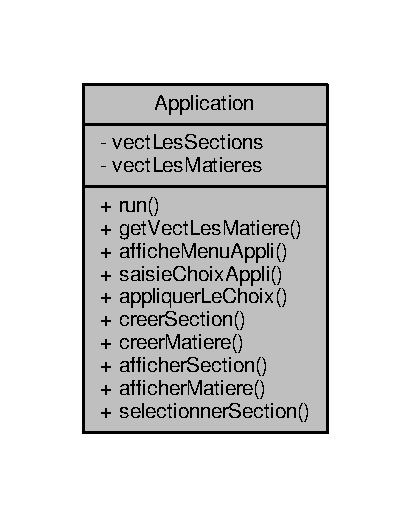
\includegraphics[width=197pt]{class_application__coll__graph}
\end{center}
\end{figure}
\subsection*{Public Member Functions}
\begin{DoxyCompactItemize}
\item 
void \hyperlink{class_application_a68965449404743bf1add056784d6cf81}{run} ()
\item 
vector$<$ \hyperlink{class_matiere}{Matiere} $>$ \hyperlink{class_application_a2aa1a9c2e0c773e3817acb4c8ff87f1d}{get\+Vect\+Les\+Matiere} ()
\begin{DoxyCompactList}\small\item\em Permet a la classe section de recuperer les differente matiere de l'application. \end{DoxyCompactList}\item 
void \hyperlink{class_application_a0c235075ac547b2cdec2e9fb8549747d}{affiche\+Menu\+Appli} ()
\begin{DoxyCompactList}\small\item\em Afficher les menu de l'application en fonction des matieres et des sections enregistrées. \end{DoxyCompactList}\item 
char \hyperlink{class_application_a9e50be67265ccc03145ed69305fc86f5}{saisie\+Choix\+Appli} ()
\item 
void \hyperlink{class_application_a48c55a5716d6731fe6191881f692e57d}{appliquer\+Le\+Choix} (char le\+Choix)
\begin{DoxyCompactList}\small\item\em Exectute l'action lier au choix de l'utilisateur. \end{DoxyCompactList}\item 
void \hyperlink{class_application_a4a0c001b058e6ff628e38bce5cc6c56b}{creer\+Section} ()
\begin{DoxyCompactList}\small\item\em Permet a l'utilisateur de créer une nouvelle section dans l'application. \end{DoxyCompactList}\item 
void \hyperlink{class_application_aea20c849e7ce31bf60b091b45e631de7}{creer\+Matiere} ()
\begin{DoxyCompactList}\small\item\em Permet a l'utilisateur de créer une nouvelle matiere dans l'application. \end{DoxyCompactList}\item 
void \hyperlink{class_application_a680db3e1303890352806d7a7e9be5601}{afficher\+Section} ()
\begin{DoxyCompactList}\small\item\em Permet a l'utilisateur d'afficher toute les sections stocker dans l'application. \end{DoxyCompactList}\item 
void \hyperlink{class_application_a00c25305470d86eedca9345b9a714ca0}{afficher\+Matiere} ()
\begin{DoxyCompactList}\small\item\em Permet a l'utilisateur d'afficher toute les matieres stocker dans l'application. \end{DoxyCompactList}\item 
void \hyperlink{class_application_ad71a2751bd07f7318be311b8128f4c3f}{selectionner\+Section} ()
\begin{DoxyCompactList}\small\item\em Permet a l'utilisateur de selectionner une section parmis toute celle renseigner dans l'application afin d'acceder a son menu. \end{DoxyCompactList}\end{DoxyCompactItemize}
\subsection*{Private Attributes}
\begin{DoxyCompactItemize}
\item 
vector$<$ \hyperlink{class_section}{Section} $>$ \hyperlink{class_application_afcbd29699ca1631db2798a23ccb5a663}{vect\+Les\+Sections}
\begin{DoxyCompactList}\small\item\em Conteneur des sections contient l'ensemble section ajouter par l'utilisateur. \end{DoxyCompactList}\item 
vector$<$ \hyperlink{class_matiere}{Matiere} $>$ \hyperlink{class_application_ac89cdfc35f9f6b669fc56fda66f97757}{vect\+Les\+Matieres}
\begin{DoxyCompactList}\small\item\em Conteneur des matieres contient toute les matieres enregistrées par l'utilisateurs. \end{DoxyCompactList}\end{DoxyCompactItemize}


\subsection{Member Function Documentation}
\hypertarget{class_application_a0c235075ac547b2cdec2e9fb8549747d}{\index{Application@{Application}!affiche\+Menu\+Appli@{affiche\+Menu\+Appli}}
\index{affiche\+Menu\+Appli@{affiche\+Menu\+Appli}!Application@{Application}}
\subsubsection[{affiche\+Menu\+Appli}]{\setlength{\rightskip}{0pt plus 5cm}Application\+::affiche\+Menu\+Appli (
\begin{DoxyParamCaption}
{}
\end{DoxyParamCaption}
)}}\label{class_application_a0c235075ac547b2cdec2e9fb8549747d}


Afficher les menu de l'application en fonction des matieres et des sections enregistrées. 

\hypertarget{class_application_a00c25305470d86eedca9345b9a714ca0}{\index{Application@{Application}!afficher\+Matiere@{afficher\+Matiere}}
\index{afficher\+Matiere@{afficher\+Matiere}!Application@{Application}}
\subsubsection[{afficher\+Matiere}]{\setlength{\rightskip}{0pt plus 5cm}Application\+::afficher\+Matiere (
\begin{DoxyParamCaption}
{}
\end{DoxyParamCaption}
)}}\label{class_application_a00c25305470d86eedca9345b9a714ca0}


Permet a l'utilisateur d'afficher toute les matieres stocker dans l'application. 

\hypertarget{class_application_a680db3e1303890352806d7a7e9be5601}{\index{Application@{Application}!afficher\+Section@{afficher\+Section}}
\index{afficher\+Section@{afficher\+Section}!Application@{Application}}
\subsubsection[{afficher\+Section}]{\setlength{\rightskip}{0pt plus 5cm}Application\+::afficher\+Section (
\begin{DoxyParamCaption}
{}
\end{DoxyParamCaption}
)}}\label{class_application_a680db3e1303890352806d7a7e9be5601}


Permet a l'utilisateur d'afficher toute les sections stocker dans l'application. 

\hypertarget{class_application_a48c55a5716d6731fe6191881f692e57d}{\index{Application@{Application}!appliquer\+Le\+Choix@{appliquer\+Le\+Choix}}
\index{appliquer\+Le\+Choix@{appliquer\+Le\+Choix}!Application@{Application}}
\subsubsection[{appliquer\+Le\+Choix}]{\setlength{\rightskip}{0pt plus 5cm}Application\+::appliquer\+Le\+Choix (
\begin{DoxyParamCaption}
\item[{char}]{le\+Choix}
\end{DoxyParamCaption}
)}}\label{class_application_a48c55a5716d6731fe6191881f692e57d}


Exectute l'action lier au choix de l'utilisateur. 

\hypertarget{class_application_aea20c849e7ce31bf60b091b45e631de7}{\index{Application@{Application}!creer\+Matiere@{creer\+Matiere}}
\index{creer\+Matiere@{creer\+Matiere}!Application@{Application}}
\subsubsection[{creer\+Matiere}]{\setlength{\rightskip}{0pt plus 5cm}Application\+::creer\+Matiere (
\begin{DoxyParamCaption}
{}
\end{DoxyParamCaption}
)}}\label{class_application_aea20c849e7ce31bf60b091b45e631de7}


Permet a l'utilisateur de créer une nouvelle matiere dans l'application. 

\hypertarget{class_application_a4a0c001b058e6ff628e38bce5cc6c56b}{\index{Application@{Application}!creer\+Section@{creer\+Section}}
\index{creer\+Section@{creer\+Section}!Application@{Application}}
\subsubsection[{creer\+Section}]{\setlength{\rightskip}{0pt plus 5cm}Application\+::creer\+Section (
\begin{DoxyParamCaption}
{}
\end{DoxyParamCaption}
)}}\label{class_application_a4a0c001b058e6ff628e38bce5cc6c56b}


Permet a l'utilisateur de créer une nouvelle section dans l'application. 

\hypertarget{class_application_a2aa1a9c2e0c773e3817acb4c8ff87f1d}{\index{Application@{Application}!get\+Vect\+Les\+Matiere@{get\+Vect\+Les\+Matiere}}
\index{get\+Vect\+Les\+Matiere@{get\+Vect\+Les\+Matiere}!Application@{Application}}
\subsubsection[{get\+Vect\+Les\+Matiere}]{\setlength{\rightskip}{0pt plus 5cm}vector$<$ {\bf Matiere} $>$ Application\+::get\+Vect\+Les\+Matiere (
\begin{DoxyParamCaption}
{}
\end{DoxyParamCaption}
)}}\label{class_application_a2aa1a9c2e0c773e3817acb4c8ff87f1d}


Permet a la classe section de recuperer les differente matiere de l'application. 

\begin{DoxyReturn}{Returns}
vect\+Les\+Matiere 
\end{DoxyReturn}
\hypertarget{class_application_a68965449404743bf1add056784d6cf81}{\index{Application@{Application}!run@{run}}
\index{run@{run}!Application@{Application}}
\subsubsection[{run}]{\setlength{\rightskip}{0pt plus 5cm}void Application\+::run (
\begin{DoxyParamCaption}
{}
\end{DoxyParamCaption}
)}}\label{class_application_a68965449404743bf1add056784d6cf81}
\hypertarget{class_application_a9e50be67265ccc03145ed69305fc86f5}{\index{Application@{Application}!saisie\+Choix\+Appli@{saisie\+Choix\+Appli}}
\index{saisie\+Choix\+Appli@{saisie\+Choix\+Appli}!Application@{Application}}
\subsubsection[{saisie\+Choix\+Appli}]{\setlength{\rightskip}{0pt plus 5cm}Application\+::saisie\+Choix\+Appli (
\begin{DoxyParamCaption}
{}
\end{DoxyParamCaption}
)}}\label{class_application_a9e50be67265ccc03145ed69305fc86f5}
\begin{DoxyReturn}{Returns}
Le choix saisie pas l'utilisateur 
\end{DoxyReturn}
\hypertarget{class_application_ad71a2751bd07f7318be311b8128f4c3f}{\index{Application@{Application}!selectionner\+Section@{selectionner\+Section}}
\index{selectionner\+Section@{selectionner\+Section}!Application@{Application}}
\subsubsection[{selectionner\+Section}]{\setlength{\rightskip}{0pt plus 5cm}Application\+::selectionner\+Section (
\begin{DoxyParamCaption}
{}
\end{DoxyParamCaption}
)}}\label{class_application_ad71a2751bd07f7318be311b8128f4c3f}


Permet a l'utilisateur de selectionner une section parmis toute celle renseigner dans l'application afin d'acceder a son menu. 



\subsection{Member Data Documentation}
\hypertarget{class_application_ac89cdfc35f9f6b669fc56fda66f97757}{\index{Application@{Application}!vect\+Les\+Matieres@{vect\+Les\+Matieres}}
\index{vect\+Les\+Matieres@{vect\+Les\+Matieres}!Application@{Application}}
\subsubsection[{vect\+Les\+Matieres}]{\setlength{\rightskip}{0pt plus 5cm}vector$<${\bf Matiere}$>$ Application\+::vect\+Les\+Matieres\hspace{0.3cm}{\ttfamily [private]}}}\label{class_application_ac89cdfc35f9f6b669fc56fda66f97757}


Conteneur des matieres contient toute les matieres enregistrées par l'utilisateurs. 

\hypertarget{class_application_afcbd29699ca1631db2798a23ccb5a663}{\index{Application@{Application}!vect\+Les\+Sections@{vect\+Les\+Sections}}
\index{vect\+Les\+Sections@{vect\+Les\+Sections}!Application@{Application}}
\subsubsection[{vect\+Les\+Sections}]{\setlength{\rightskip}{0pt plus 5cm}vector$<${\bf Section}$>$ Application\+::vect\+Les\+Sections\hspace{0.3cm}{\ttfamily [private]}}}\label{class_application_afcbd29699ca1631db2798a23ccb5a663}


Conteneur des sections contient l'ensemble section ajouter par l'utilisateur. 



The documentation for this class was generated from the following files\+:\begin{DoxyCompactItemize}
\item 
\hyperlink{application_8h}{application.\+h}\item 
\hyperlink{application_8cpp}{application.\+cpp}\end{DoxyCompactItemize}

\hypertarget{class_bulletin}{\section{Bulletin Class Reference}
\label{class_bulletin}\index{Bulletin@{Bulletin}}
}


{\ttfamily \#include $<$bulletin.\+h$>$}



Collaboration diagram for Bulletin\+:\nopagebreak
\begin{figure}[H]
\begin{center}
\leavevmode
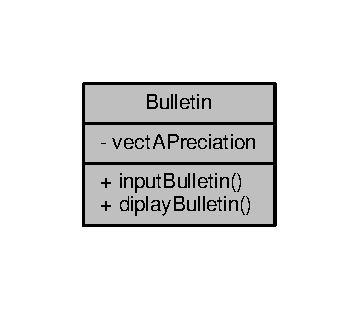
\includegraphics[width=172pt]{class_bulletin__coll__graph}
\end{center}
\end{figure}
\subsection*{Public Member Functions}
\begin{DoxyCompactItemize}
\item 
void \hyperlink{class_bulletin_ac116403c81f034712bf7cf41a281d650}{input\+Bulletin} ()
\item 
void \hyperlink{class_bulletin_aeb581b55746121f5eee9b23c0ef64804}{diplay\+Bulletin} ()
\end{DoxyCompactItemize}
\subsection*{Private Attributes}
\begin{DoxyCompactItemize}
\item 
vector$<$ string $>$ \hyperlink{class_bulletin_ac2ebf9657e81664fa0811f0aaccf825c}{vect\+A\+Preciation}
\end{DoxyCompactItemize}


\subsection{Member Function Documentation}
\hypertarget{class_bulletin_aeb581b55746121f5eee9b23c0ef64804}{\index{Bulletin@{Bulletin}!diplay\+Bulletin@{diplay\+Bulletin}}
\index{diplay\+Bulletin@{diplay\+Bulletin}!Bulletin@{Bulletin}}
\subsubsection[{diplay\+Bulletin}]{\setlength{\rightskip}{0pt plus 5cm}void Bulletin\+::diplay\+Bulletin (
\begin{DoxyParamCaption}
{}
\end{DoxyParamCaption}
)}}\label{class_bulletin_aeb581b55746121f5eee9b23c0ef64804}
\hypertarget{class_bulletin_ac116403c81f034712bf7cf41a281d650}{\index{Bulletin@{Bulletin}!input\+Bulletin@{input\+Bulletin}}
\index{input\+Bulletin@{input\+Bulletin}!Bulletin@{Bulletin}}
\subsubsection[{input\+Bulletin}]{\setlength{\rightskip}{0pt plus 5cm}void Bulletin\+::input\+Bulletin (
\begin{DoxyParamCaption}
{}
\end{DoxyParamCaption}
)}}\label{class_bulletin_ac116403c81f034712bf7cf41a281d650}


\subsection{Member Data Documentation}
\hypertarget{class_bulletin_ac2ebf9657e81664fa0811f0aaccf825c}{\index{Bulletin@{Bulletin}!vect\+A\+Preciation@{vect\+A\+Preciation}}
\index{vect\+A\+Preciation@{vect\+A\+Preciation}!Bulletin@{Bulletin}}
\subsubsection[{vect\+A\+Preciation}]{\setlength{\rightskip}{0pt plus 5cm}vector$<$string$>$ Bulletin\+::vect\+A\+Preciation\hspace{0.3cm}{\ttfamily [private]}}}\label{class_bulletin_ac2ebf9657e81664fa0811f0aaccf825c}


The documentation for this class was generated from the following file\+:\begin{DoxyCompactItemize}
\item 
\hyperlink{bulletin_8h}{bulletin.\+h}\end{DoxyCompactItemize}

\hypertarget{class_eleve}{\section{Eleve Class Reference}
\label{class_eleve}\index{Eleve@{Eleve}}
}


{\ttfamily \#include $<$eleve.\+h$>$}



Collaboration diagram for Eleve\+:\nopagebreak
\begin{figure}[H]
\begin{center}
\leavevmode
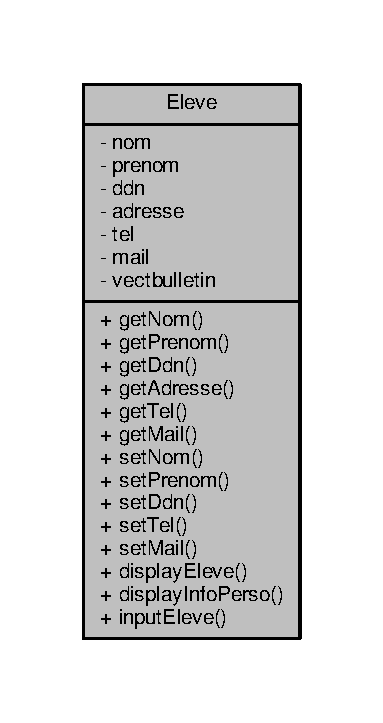
\includegraphics[width=184pt]{class_eleve__coll__graph}
\end{center}
\end{figure}
\subsection*{Public Member Functions}
\begin{DoxyCompactItemize}
\item 
string \hyperlink{class_eleve_abf63239397983c10c4dfea36839aa522}{get\+Nom} ()
\item 
string \hyperlink{class_eleve_a306ededf39fac45344ceb81f4591d96f}{get\+Prenom} ()
\item 
string \hyperlink{class_eleve_a763cd01d1dd01ab767993af4cddd2287}{get\+Ddn} ()
\item 
string \hyperlink{class_eleve_a6e116a71d9ff92a800924bb007071695}{get\+Adresse} ()
\item 
string \hyperlink{class_eleve_a654c5306631f47e2935d6bb824103dad}{get\+Tel} ()
\item 
string \hyperlink{class_eleve_acc6dd85cc1a1772ec64452d4de335c75}{get\+Mail} ()
\item 
void \hyperlink{class_eleve_a020452a09dac3e0c71f733ab6076ad26}{set\+Nom} (string le\+Nom)
\item 
void \hyperlink{class_eleve_a680c0bc086177e18c058347f88e76919}{set\+Prenom} (string le\+Prenom)
\item 
void \hyperlink{class_eleve_aa59d7a77676c74d319fc192b052db3be}{set\+Ddn} (string la\+Ddn)
\item 
void \hyperlink{class_eleve_a5551f7974770c2a532d460e90707a8ec}{set\+Tel} (string le\+Tel)
\item 
void \hyperlink{class_eleve_aa7fe74f0d1328aae34effbbf465b4173}{set\+Mail} (string le\+Mail)
\item 
void \hyperlink{class_eleve_a8c7b5d6cdec71c14fc4f05d669d3e7d4}{display\+Eleve} ()
\item 
void \hyperlink{class_eleve_a6fff5d0f8829381a5623384b0f4b0791}{display\+Info\+Perso} ()
\item 
void \hyperlink{class_eleve_ab2ee2e1f243c9ebfeca5c21852874b8f}{input\+Eleve} ()
\end{DoxyCompactItemize}
\subsection*{Private Attributes}
\begin{DoxyCompactItemize}
\item 
string \hyperlink{class_eleve_a912b79db853e8dd2e0fd5c9f0fae1986}{nom}
\item 
string \hyperlink{class_eleve_a751fd312c37f99b67b13dccf3e017f00}{prenom}
\item 
string \hyperlink{class_eleve_af66f74f6f47e1d9d548f4ea583181050}{ddn}
\item 
string \hyperlink{class_eleve_a397780b74849d969b9095457dba8e1c1}{adresse}
\item 
string \hyperlink{class_eleve_a4dbaefdec13d5feabd6c98eea3af84c1}{tel}
\item 
string \hyperlink{class_eleve_a55582aa568fa4bbbb3f7d151e49e4709}{mail}
\item 
vector$<$ \hyperlink{class_bulletin}{Bulletin} $>$ \hyperlink{class_eleve_ac5a4dd1b22caf00a6b055184b10b734d}{vectbulletin}
\end{DoxyCompactItemize}


\subsection{Member Function Documentation}
\hypertarget{class_eleve_a8c7b5d6cdec71c14fc4f05d669d3e7d4}{\index{Eleve@{Eleve}!display\+Eleve@{display\+Eleve}}
\index{display\+Eleve@{display\+Eleve}!Eleve@{Eleve}}
\subsubsection[{display\+Eleve}]{\setlength{\rightskip}{0pt plus 5cm}void Eleve\+::display\+Eleve (
\begin{DoxyParamCaption}
{}
\end{DoxyParamCaption}
)}}\label{class_eleve_a8c7b5d6cdec71c14fc4f05d669d3e7d4}
\hypertarget{class_eleve_a6fff5d0f8829381a5623384b0f4b0791}{\index{Eleve@{Eleve}!display\+Info\+Perso@{display\+Info\+Perso}}
\index{display\+Info\+Perso@{display\+Info\+Perso}!Eleve@{Eleve}}
\subsubsection[{display\+Info\+Perso}]{\setlength{\rightskip}{0pt plus 5cm}void Eleve\+::display\+Info\+Perso (
\begin{DoxyParamCaption}
{}
\end{DoxyParamCaption}
)}}\label{class_eleve_a6fff5d0f8829381a5623384b0f4b0791}
\hypertarget{class_eleve_a6e116a71d9ff92a800924bb007071695}{\index{Eleve@{Eleve}!get\+Adresse@{get\+Adresse}}
\index{get\+Adresse@{get\+Adresse}!Eleve@{Eleve}}
\subsubsection[{get\+Adresse}]{\setlength{\rightskip}{0pt plus 5cm}string Eleve\+::get\+Adresse (
\begin{DoxyParamCaption}
{}
\end{DoxyParamCaption}
)}}\label{class_eleve_a6e116a71d9ff92a800924bb007071695}
\hypertarget{class_eleve_a763cd01d1dd01ab767993af4cddd2287}{\index{Eleve@{Eleve}!get\+Ddn@{get\+Ddn}}
\index{get\+Ddn@{get\+Ddn}!Eleve@{Eleve}}
\subsubsection[{get\+Ddn}]{\setlength{\rightskip}{0pt plus 5cm}string Eleve\+::get\+Ddn (
\begin{DoxyParamCaption}
{}
\end{DoxyParamCaption}
)}}\label{class_eleve_a763cd01d1dd01ab767993af4cddd2287}
\hypertarget{class_eleve_acc6dd85cc1a1772ec64452d4de335c75}{\index{Eleve@{Eleve}!get\+Mail@{get\+Mail}}
\index{get\+Mail@{get\+Mail}!Eleve@{Eleve}}
\subsubsection[{get\+Mail}]{\setlength{\rightskip}{0pt plus 5cm}string Eleve\+::get\+Mail (
\begin{DoxyParamCaption}
{}
\end{DoxyParamCaption}
)}}\label{class_eleve_acc6dd85cc1a1772ec64452d4de335c75}
\hypertarget{class_eleve_abf63239397983c10c4dfea36839aa522}{\index{Eleve@{Eleve}!get\+Nom@{get\+Nom}}
\index{get\+Nom@{get\+Nom}!Eleve@{Eleve}}
\subsubsection[{get\+Nom}]{\setlength{\rightskip}{0pt plus 5cm}string Eleve\+::get\+Nom (
\begin{DoxyParamCaption}
{}
\end{DoxyParamCaption}
)}}\label{class_eleve_abf63239397983c10c4dfea36839aa522}
\hypertarget{class_eleve_a306ededf39fac45344ceb81f4591d96f}{\index{Eleve@{Eleve}!get\+Prenom@{get\+Prenom}}
\index{get\+Prenom@{get\+Prenom}!Eleve@{Eleve}}
\subsubsection[{get\+Prenom}]{\setlength{\rightskip}{0pt plus 5cm}string Eleve\+::get\+Prenom (
\begin{DoxyParamCaption}
{}
\end{DoxyParamCaption}
)}}\label{class_eleve_a306ededf39fac45344ceb81f4591d96f}
\hypertarget{class_eleve_a654c5306631f47e2935d6bb824103dad}{\index{Eleve@{Eleve}!get\+Tel@{get\+Tel}}
\index{get\+Tel@{get\+Tel}!Eleve@{Eleve}}
\subsubsection[{get\+Tel}]{\setlength{\rightskip}{0pt plus 5cm}string Eleve\+::get\+Tel (
\begin{DoxyParamCaption}
{}
\end{DoxyParamCaption}
)}}\label{class_eleve_a654c5306631f47e2935d6bb824103dad}
\hypertarget{class_eleve_ab2ee2e1f243c9ebfeca5c21852874b8f}{\index{Eleve@{Eleve}!input\+Eleve@{input\+Eleve}}
\index{input\+Eleve@{input\+Eleve}!Eleve@{Eleve}}
\subsubsection[{input\+Eleve}]{\setlength{\rightskip}{0pt plus 5cm}void Eleve\+::input\+Eleve (
\begin{DoxyParamCaption}
{}
\end{DoxyParamCaption}
)}}\label{class_eleve_ab2ee2e1f243c9ebfeca5c21852874b8f}
\hypertarget{class_eleve_aa59d7a77676c74d319fc192b052db3be}{\index{Eleve@{Eleve}!set\+Ddn@{set\+Ddn}}
\index{set\+Ddn@{set\+Ddn}!Eleve@{Eleve}}
\subsubsection[{set\+Ddn}]{\setlength{\rightskip}{0pt plus 5cm}void Eleve\+::set\+Ddn (
\begin{DoxyParamCaption}
\item[{string}]{la\+Ddn}
\end{DoxyParamCaption}
)}}\label{class_eleve_aa59d7a77676c74d319fc192b052db3be}
\hypertarget{class_eleve_aa7fe74f0d1328aae34effbbf465b4173}{\index{Eleve@{Eleve}!set\+Mail@{set\+Mail}}
\index{set\+Mail@{set\+Mail}!Eleve@{Eleve}}
\subsubsection[{set\+Mail}]{\setlength{\rightskip}{0pt plus 5cm}void Eleve\+::set\+Mail (
\begin{DoxyParamCaption}
\item[{string}]{le\+Mail}
\end{DoxyParamCaption}
)}}\label{class_eleve_aa7fe74f0d1328aae34effbbf465b4173}
\hypertarget{class_eleve_a020452a09dac3e0c71f733ab6076ad26}{\index{Eleve@{Eleve}!set\+Nom@{set\+Nom}}
\index{set\+Nom@{set\+Nom}!Eleve@{Eleve}}
\subsubsection[{set\+Nom}]{\setlength{\rightskip}{0pt plus 5cm}void Eleve\+::set\+Nom (
\begin{DoxyParamCaption}
\item[{string}]{le\+Nom}
\end{DoxyParamCaption}
)}}\label{class_eleve_a020452a09dac3e0c71f733ab6076ad26}
\hypertarget{class_eleve_a680c0bc086177e18c058347f88e76919}{\index{Eleve@{Eleve}!set\+Prenom@{set\+Prenom}}
\index{set\+Prenom@{set\+Prenom}!Eleve@{Eleve}}
\subsubsection[{set\+Prenom}]{\setlength{\rightskip}{0pt plus 5cm}void Eleve\+::set\+Prenom (
\begin{DoxyParamCaption}
\item[{string}]{le\+Prenom}
\end{DoxyParamCaption}
)}}\label{class_eleve_a680c0bc086177e18c058347f88e76919}
\hypertarget{class_eleve_a5551f7974770c2a532d460e90707a8ec}{\index{Eleve@{Eleve}!set\+Tel@{set\+Tel}}
\index{set\+Tel@{set\+Tel}!Eleve@{Eleve}}
\subsubsection[{set\+Tel}]{\setlength{\rightskip}{0pt plus 5cm}void Eleve\+::set\+Tel (
\begin{DoxyParamCaption}
\item[{string}]{le\+Tel}
\end{DoxyParamCaption}
)}}\label{class_eleve_a5551f7974770c2a532d460e90707a8ec}


\subsection{Member Data Documentation}
\hypertarget{class_eleve_a397780b74849d969b9095457dba8e1c1}{\index{Eleve@{Eleve}!adresse@{adresse}}
\index{adresse@{adresse}!Eleve@{Eleve}}
\subsubsection[{adresse}]{\setlength{\rightskip}{0pt plus 5cm}string Eleve\+::adresse\hspace{0.3cm}{\ttfamily [private]}}}\label{class_eleve_a397780b74849d969b9095457dba8e1c1}
\hypertarget{class_eleve_af66f74f6f47e1d9d548f4ea583181050}{\index{Eleve@{Eleve}!ddn@{ddn}}
\index{ddn@{ddn}!Eleve@{Eleve}}
\subsubsection[{ddn}]{\setlength{\rightskip}{0pt plus 5cm}string Eleve\+::ddn\hspace{0.3cm}{\ttfamily [private]}}}\label{class_eleve_af66f74f6f47e1d9d548f4ea583181050}
\hypertarget{class_eleve_a55582aa568fa4bbbb3f7d151e49e4709}{\index{Eleve@{Eleve}!mail@{mail}}
\index{mail@{mail}!Eleve@{Eleve}}
\subsubsection[{mail}]{\setlength{\rightskip}{0pt plus 5cm}string Eleve\+::mail\hspace{0.3cm}{\ttfamily [private]}}}\label{class_eleve_a55582aa568fa4bbbb3f7d151e49e4709}
\hypertarget{class_eleve_a912b79db853e8dd2e0fd5c9f0fae1986}{\index{Eleve@{Eleve}!nom@{nom}}
\index{nom@{nom}!Eleve@{Eleve}}
\subsubsection[{nom}]{\setlength{\rightskip}{0pt plus 5cm}string Eleve\+::nom\hspace{0.3cm}{\ttfamily [private]}}}\label{class_eleve_a912b79db853e8dd2e0fd5c9f0fae1986}
\hypertarget{class_eleve_a751fd312c37f99b67b13dccf3e017f00}{\index{Eleve@{Eleve}!prenom@{prenom}}
\index{prenom@{prenom}!Eleve@{Eleve}}
\subsubsection[{prenom}]{\setlength{\rightskip}{0pt plus 5cm}string Eleve\+::prenom\hspace{0.3cm}{\ttfamily [private]}}}\label{class_eleve_a751fd312c37f99b67b13dccf3e017f00}
\hypertarget{class_eleve_a4dbaefdec13d5feabd6c98eea3af84c1}{\index{Eleve@{Eleve}!tel@{tel}}
\index{tel@{tel}!Eleve@{Eleve}}
\subsubsection[{tel}]{\setlength{\rightskip}{0pt plus 5cm}string Eleve\+::tel\hspace{0.3cm}{\ttfamily [private]}}}\label{class_eleve_a4dbaefdec13d5feabd6c98eea3af84c1}
\hypertarget{class_eleve_ac5a4dd1b22caf00a6b055184b10b734d}{\index{Eleve@{Eleve}!vectbulletin@{vectbulletin}}
\index{vectbulletin@{vectbulletin}!Eleve@{Eleve}}
\subsubsection[{vectbulletin}]{\setlength{\rightskip}{0pt plus 5cm}vector$<${\bf Bulletin}$>$ Eleve\+::vectbulletin\hspace{0.3cm}{\ttfamily [private]}}}\label{class_eleve_ac5a4dd1b22caf00a6b055184b10b734d}


The documentation for this class was generated from the following files\+:\begin{DoxyCompactItemize}
\item 
\hyperlink{eleve_8h}{eleve.\+h}\item 
\hyperlink{eleve_8cpp}{eleve.\+cpp}\end{DoxyCompactItemize}

\hypertarget{class_evaluation}{\section{Evaluation Class Reference}
\label{class_evaluation}\index{Evaluation@{Evaluation}}
}


{\ttfamily \#include $<$evaluation.\+h$>$}



Collaboration diagram for Evaluation\+:\nopagebreak
\begin{figure}[H]
\begin{center}
\leavevmode
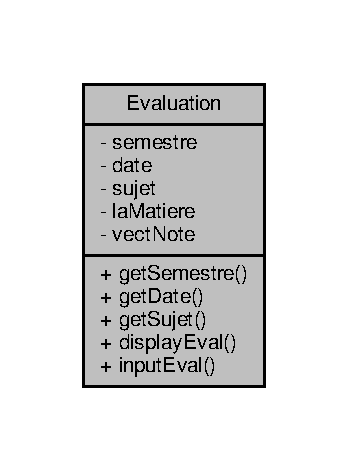
\includegraphics[width=167pt]{class_evaluation__coll__graph}
\end{center}
\end{figure}
\subsection*{Public Member Functions}
\begin{DoxyCompactItemize}
\item 
int \hyperlink{class_evaluation_aa6dd5cebc7176c567c8da59d0e03a552}{get\+Semestre} ()
\item 
string \hyperlink{class_evaluation_a737df75c5f979ec212554209f9224a6e}{get\+Date} ()
\item 
string \hyperlink{class_evaluation_a715aaa51b427078b85a4b68fda0c4baf}{get\+Sujet} ()
\item 
void \hyperlink{class_evaluation_ad2236e7c0ca268589ba9394a179ee532}{display\+Eval} ()
\item 
void \hyperlink{class_evaluation_a76c6aa88b472baae9afbc911a9faf179}{input\+Eval} ()
\end{DoxyCompactItemize}
\subsection*{Private Attributes}
\begin{DoxyCompactItemize}
\item 
int \hyperlink{class_evaluation_ae000ec143562ed56975018bf82b13b5c}{semestre}
\item 
string \hyperlink{class_evaluation_af97cdd68e574cc998f161f83c0f6b855}{date}
\item 
string \hyperlink{class_evaluation_a03ed74f0b6d6b28f3ac877312e3cbd8a}{sujet}
\item 
vector$<$ \hyperlink{class_matiere}{Matiere} $\ast$ $>$ \hyperlink{class_evaluation_a28a58ead557883cd0d51af79d2f2d42a}{la\+Matiere}
\item 
vector$<$ \hyperlink{class_note}{Note} $>$ \hyperlink{class_evaluation_ad26840cec05aea45af3b1164c55a7557}{vect\+Note}
\end{DoxyCompactItemize}


\subsection{Member Function Documentation}
\hypertarget{class_evaluation_ad2236e7c0ca268589ba9394a179ee532}{\index{Evaluation@{Evaluation}!display\+Eval@{display\+Eval}}
\index{display\+Eval@{display\+Eval}!Evaluation@{Evaluation}}
\subsubsection[{display\+Eval}]{\setlength{\rightskip}{0pt plus 5cm}void Evaluation\+::display\+Eval (
\begin{DoxyParamCaption}
{}
\end{DoxyParamCaption}
)}}\label{class_evaluation_ad2236e7c0ca268589ba9394a179ee532}
\hypertarget{class_evaluation_a737df75c5f979ec212554209f9224a6e}{\index{Evaluation@{Evaluation}!get\+Date@{get\+Date}}
\index{get\+Date@{get\+Date}!Evaluation@{Evaluation}}
\subsubsection[{get\+Date}]{\setlength{\rightskip}{0pt plus 5cm}string Evaluation\+::get\+Date (
\begin{DoxyParamCaption}
{}
\end{DoxyParamCaption}
)}}\label{class_evaluation_a737df75c5f979ec212554209f9224a6e}
\hypertarget{class_evaluation_aa6dd5cebc7176c567c8da59d0e03a552}{\index{Evaluation@{Evaluation}!get\+Semestre@{get\+Semestre}}
\index{get\+Semestre@{get\+Semestre}!Evaluation@{Evaluation}}
\subsubsection[{get\+Semestre}]{\setlength{\rightskip}{0pt plus 5cm}int Evaluation\+::get\+Semestre (
\begin{DoxyParamCaption}
{}
\end{DoxyParamCaption}
)}}\label{class_evaluation_aa6dd5cebc7176c567c8da59d0e03a552}
\hypertarget{class_evaluation_a715aaa51b427078b85a4b68fda0c4baf}{\index{Evaluation@{Evaluation}!get\+Sujet@{get\+Sujet}}
\index{get\+Sujet@{get\+Sujet}!Evaluation@{Evaluation}}
\subsubsection[{get\+Sujet}]{\setlength{\rightskip}{0pt plus 5cm}string Evaluation\+::get\+Sujet (
\begin{DoxyParamCaption}
{}
\end{DoxyParamCaption}
)}}\label{class_evaluation_a715aaa51b427078b85a4b68fda0c4baf}
\hypertarget{class_evaluation_a76c6aa88b472baae9afbc911a9faf179}{\index{Evaluation@{Evaluation}!input\+Eval@{input\+Eval}}
\index{input\+Eval@{input\+Eval}!Evaluation@{Evaluation}}
\subsubsection[{input\+Eval}]{\setlength{\rightskip}{0pt plus 5cm}void Evaluation\+::input\+Eval (
\begin{DoxyParamCaption}
{}
\end{DoxyParamCaption}
)}}\label{class_evaluation_a76c6aa88b472baae9afbc911a9faf179}


\subsection{Member Data Documentation}
\hypertarget{class_evaluation_af97cdd68e574cc998f161f83c0f6b855}{\index{Evaluation@{Evaluation}!date@{date}}
\index{date@{date}!Evaluation@{Evaluation}}
\subsubsection[{date}]{\setlength{\rightskip}{0pt plus 5cm}string Evaluation\+::date\hspace{0.3cm}{\ttfamily [private]}}}\label{class_evaluation_af97cdd68e574cc998f161f83c0f6b855}
\hypertarget{class_evaluation_a28a58ead557883cd0d51af79d2f2d42a}{\index{Evaluation@{Evaluation}!la\+Matiere@{la\+Matiere}}
\index{la\+Matiere@{la\+Matiere}!Evaluation@{Evaluation}}
\subsubsection[{la\+Matiere}]{\setlength{\rightskip}{0pt plus 5cm}vector$<${\bf Matiere}$\ast$$>$ Evaluation\+::la\+Matiere\hspace{0.3cm}{\ttfamily [private]}}}\label{class_evaluation_a28a58ead557883cd0d51af79d2f2d42a}
\hypertarget{class_evaluation_ae000ec143562ed56975018bf82b13b5c}{\index{Evaluation@{Evaluation}!semestre@{semestre}}
\index{semestre@{semestre}!Evaluation@{Evaluation}}
\subsubsection[{semestre}]{\setlength{\rightskip}{0pt plus 5cm}int Evaluation\+::semestre\hspace{0.3cm}{\ttfamily [private]}}}\label{class_evaluation_ae000ec143562ed56975018bf82b13b5c}
\hypertarget{class_evaluation_a03ed74f0b6d6b28f3ac877312e3cbd8a}{\index{Evaluation@{Evaluation}!sujet@{sujet}}
\index{sujet@{sujet}!Evaluation@{Evaluation}}
\subsubsection[{sujet}]{\setlength{\rightskip}{0pt plus 5cm}string Evaluation\+::sujet\hspace{0.3cm}{\ttfamily [private]}}}\label{class_evaluation_a03ed74f0b6d6b28f3ac877312e3cbd8a}
\hypertarget{class_evaluation_ad26840cec05aea45af3b1164c55a7557}{\index{Evaluation@{Evaluation}!vect\+Note@{vect\+Note}}
\index{vect\+Note@{vect\+Note}!Evaluation@{Evaluation}}
\subsubsection[{vect\+Note}]{\setlength{\rightskip}{0pt plus 5cm}vector$<${\bf Note}$>$ Evaluation\+::vect\+Note\hspace{0.3cm}{\ttfamily [private]}}}\label{class_evaluation_ad26840cec05aea45af3b1164c55a7557}


The documentation for this class was generated from the following file\+:\begin{DoxyCompactItemize}
\item 
\hyperlink{evaluation_8h}{evaluation.\+h}\end{DoxyCompactItemize}

\hypertarget{class_matiere}{\section{Matiere Class Reference}
\label{class_matiere}\index{Matiere@{Matiere}}
}


{\ttfamily \#include $<$matiere.\+h$>$}



Collaboration diagram for Matiere\+:\nopagebreak
\begin{figure}[H]
\begin{center}
\leavevmode
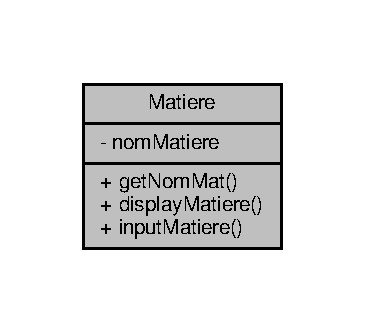
\includegraphics[width=175pt]{class_matiere__coll__graph}
\end{center}
\end{figure}
\subsection*{Public Member Functions}
\begin{DoxyCompactItemize}
\item 
string \hyperlink{class_matiere_a51db02074e8da744c8d83e21ccc87141}{get\+Nom\+Mat} ()
\item 
void \hyperlink{class_matiere_a0ad25e7a36a710e6a81e4ff2e0e1e39c}{display\+Matiere} ()
\item 
void \hyperlink{class_matiere_a5280bde49139a6cc89b4198797df6a15}{input\+Matiere} ()
\end{DoxyCompactItemize}
\subsection*{Private Attributes}
\begin{DoxyCompactItemize}
\item 
string \hyperlink{class_matiere_a701728c9283e82fd270a91a8eb541917}{nom\+Matiere}
\end{DoxyCompactItemize}


\subsection{Member Function Documentation}
\hypertarget{class_matiere_a0ad25e7a36a710e6a81e4ff2e0e1e39c}{\index{Matiere@{Matiere}!display\+Matiere@{display\+Matiere}}
\index{display\+Matiere@{display\+Matiere}!Matiere@{Matiere}}
\subsubsection[{display\+Matiere}]{\setlength{\rightskip}{0pt plus 5cm}void Matiere\+::display\+Matiere (
\begin{DoxyParamCaption}
{}
\end{DoxyParamCaption}
)}}\label{class_matiere_a0ad25e7a36a710e6a81e4ff2e0e1e39c}
\hypertarget{class_matiere_a51db02074e8da744c8d83e21ccc87141}{\index{Matiere@{Matiere}!get\+Nom\+Mat@{get\+Nom\+Mat}}
\index{get\+Nom\+Mat@{get\+Nom\+Mat}!Matiere@{Matiere}}
\subsubsection[{get\+Nom\+Mat}]{\setlength{\rightskip}{0pt plus 5cm}string Matiere\+::get\+Nom\+Mat (
\begin{DoxyParamCaption}
{}
\end{DoxyParamCaption}
)}}\label{class_matiere_a51db02074e8da744c8d83e21ccc87141}
\hypertarget{class_matiere_a5280bde49139a6cc89b4198797df6a15}{\index{Matiere@{Matiere}!input\+Matiere@{input\+Matiere}}
\index{input\+Matiere@{input\+Matiere}!Matiere@{Matiere}}
\subsubsection[{input\+Matiere}]{\setlength{\rightskip}{0pt plus 5cm}void Matiere\+::input\+Matiere (
\begin{DoxyParamCaption}
{}
\end{DoxyParamCaption}
)}}\label{class_matiere_a5280bde49139a6cc89b4198797df6a15}


\subsection{Member Data Documentation}
\hypertarget{class_matiere_a701728c9283e82fd270a91a8eb541917}{\index{Matiere@{Matiere}!nom\+Matiere@{nom\+Matiere}}
\index{nom\+Matiere@{nom\+Matiere}!Matiere@{Matiere}}
\subsubsection[{nom\+Matiere}]{\setlength{\rightskip}{0pt plus 5cm}string Matiere\+::nom\+Matiere\hspace{0.3cm}{\ttfamily [private]}}}\label{class_matiere_a701728c9283e82fd270a91a8eb541917}


The documentation for this class was generated from the following files\+:\begin{DoxyCompactItemize}
\item 
\hyperlink{matiere_8h}{matiere.\+h}\item 
\hyperlink{matiere_8cpp}{matiere.\+cpp}\end{DoxyCompactItemize}

\hypertarget{class_note}{\section{Note Class Reference}
\label{class_note}\index{Note@{Note}}
}


{\ttfamily \#include $<$note.\+h$>$}



Collaboration diagram for Note\+:\nopagebreak
\begin{figure}[H]
\begin{center}
\leavevmode
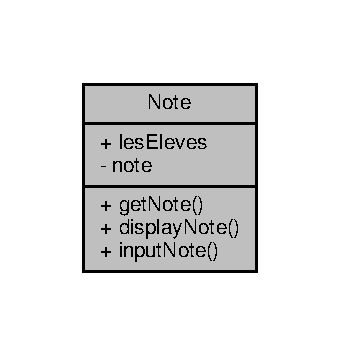
\includegraphics[width=163pt]{class_note__coll__graph}
\end{center}
\end{figure}
\subsection*{Public Member Functions}
\begin{DoxyCompactItemize}
\item 
int \hyperlink{class_note_a880f020b1e9fe974fd2a3064af3257c6}{get\+Note} ()
\item 
void \hyperlink{class_note_ae9f2d7513a834ad2198a66e50a1ba38b}{display\+Note} ()
\item 
void \hyperlink{class_note_a2232542d07b8c3657c0e43da23afaedf}{input\+Note} ()
\end{DoxyCompactItemize}
\subsection*{Public Attributes}
\begin{DoxyCompactItemize}
\item 
vector$<$ \hyperlink{class_eleve}{Eleve} $\ast$ $>$ \hyperlink{class_note_a9e61b19e4928a16b63e5dd9c4fee859b}{les\+Eleves}
\end{DoxyCompactItemize}
\subsection*{Private Attributes}
\begin{DoxyCompactItemize}
\item 
int \hyperlink{class_note_a3cb5f22dd5374f4e3c59c5f11dc7fbfb}{note}
\end{DoxyCompactItemize}


\subsection{Member Function Documentation}
\hypertarget{class_note_ae9f2d7513a834ad2198a66e50a1ba38b}{\index{Note@{Note}!display\+Note@{display\+Note}}
\index{display\+Note@{display\+Note}!Note@{Note}}
\subsubsection[{display\+Note}]{\setlength{\rightskip}{0pt plus 5cm}void Note\+::display\+Note (
\begin{DoxyParamCaption}
{}
\end{DoxyParamCaption}
)}}\label{class_note_ae9f2d7513a834ad2198a66e50a1ba38b}
\hypertarget{class_note_a880f020b1e9fe974fd2a3064af3257c6}{\index{Note@{Note}!get\+Note@{get\+Note}}
\index{get\+Note@{get\+Note}!Note@{Note}}
\subsubsection[{get\+Note}]{\setlength{\rightskip}{0pt plus 5cm}int Note\+::get\+Note (
\begin{DoxyParamCaption}
{}
\end{DoxyParamCaption}
)}}\label{class_note_a880f020b1e9fe974fd2a3064af3257c6}
\hypertarget{class_note_a2232542d07b8c3657c0e43da23afaedf}{\index{Note@{Note}!input\+Note@{input\+Note}}
\index{input\+Note@{input\+Note}!Note@{Note}}
\subsubsection[{input\+Note}]{\setlength{\rightskip}{0pt plus 5cm}void Note\+::input\+Note (
\begin{DoxyParamCaption}
{}
\end{DoxyParamCaption}
)}}\label{class_note_a2232542d07b8c3657c0e43da23afaedf}


\subsection{Member Data Documentation}
\hypertarget{class_note_a9e61b19e4928a16b63e5dd9c4fee859b}{\index{Note@{Note}!les\+Eleves@{les\+Eleves}}
\index{les\+Eleves@{les\+Eleves}!Note@{Note}}
\subsubsection[{les\+Eleves}]{\setlength{\rightskip}{0pt plus 5cm}vector$<${\bf Eleve}$\ast$$>$ Note\+::les\+Eleves}}\label{class_note_a9e61b19e4928a16b63e5dd9c4fee859b}
\hypertarget{class_note_a3cb5f22dd5374f4e3c59c5f11dc7fbfb}{\index{Note@{Note}!note@{note}}
\index{note@{note}!Note@{Note}}
\subsubsection[{note}]{\setlength{\rightskip}{0pt plus 5cm}int Note\+::note\hspace{0.3cm}{\ttfamily [private]}}}\label{class_note_a3cb5f22dd5374f4e3c59c5f11dc7fbfb}


The documentation for this class was generated from the following file\+:\begin{DoxyCompactItemize}
\item 
\hyperlink{note_8h}{note.\+h}\end{DoxyCompactItemize}

\hypertarget{class_section}{\section{Section Class Reference}
\label{class_section}\index{Section@{Section}}
}


{\ttfamily \#include $<$section.\+h$>$}



Collaboration diagram for Section\+:\nopagebreak
\begin{figure}[H]
\begin{center}
\leavevmode
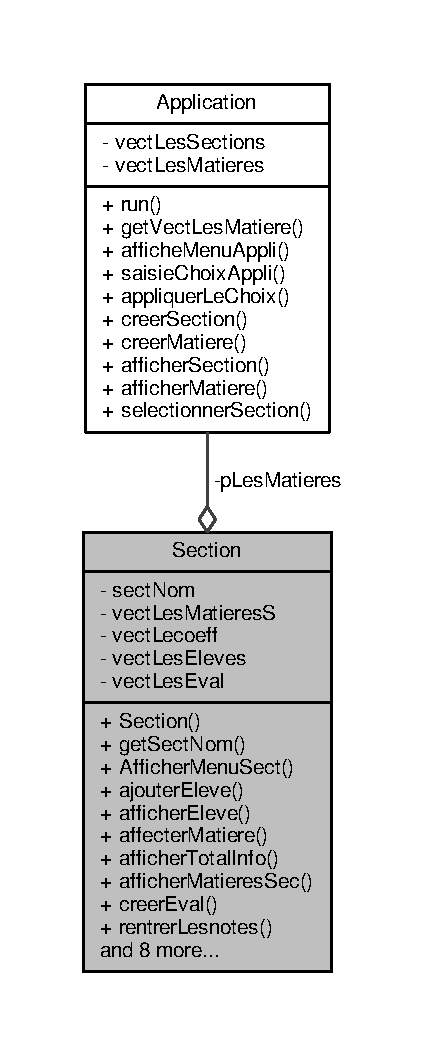
\includegraphics[width=204pt]{class_section__coll__graph}
\end{center}
\end{figure}
\subsection*{Public Member Functions}
\begin{DoxyCompactItemize}
\item 
\hyperlink{class_section_a288017c7bfd0fe6aee6e29bae921c7ee}{Section} (\hyperlink{class_application}{Application} $\ast$\hyperlink{class_matiere}{Matiere})
\item 
string \hyperlink{class_section_a33720a47c81f2380b945dec28b8e39d7}{get\+Sect\+Nom} ()
\item 
void \hyperlink{class_section_a93b414675ebd2667409a44a9b986cc4f}{Afficher\+Menu\+Sect} ()
\item 
void \hyperlink{class_section_afa8816db504195a8c1f5c9d8c3ccbd34}{ajouter\+Eleve} ()
\item 
void \hyperlink{class_section_a367d97fad77c046a78aa6dd0ce7a9315}{afficher\+Eleve} ()
\item 
void \hyperlink{class_section_a0b7c4fec05a94910766becb5291e44cb}{affecter\+Matiere} ()
\item 
void \hyperlink{class_section_a4ba7e1644f017aebc9f8721a0ede4ee6}{afficher\+Total\+Info} ()
\item 
void \hyperlink{class_section_ac6e6d0f8dafcb0854c164df62dfc2bde}{afficher\+Matieres\+Sec} ()
\item 
void \hyperlink{class_section_afeff96d837b03663d9820fc80d1479ed}{creer\+Eval} ()
\item 
void \hyperlink{class_section_a08e8460e2b2cb7b4e69564bd45c8929f}{rentrer\+Lesnotes} ()
\item 
void \hyperlink{class_section_abc1815ec698a6510d8315551bb792ea9}{afficher\+Eval\+Et\+Notes} ()
\item 
void \hyperlink{class_section_a9c8ed068a26b1c29cff8597a0a13c2ae}{creation\+Bulletin} ()
\item 
void \hyperlink{class_section_a01b0acae2cd1395aa949ff8ba18b307a}{affiche\+Menu\+Section} ()
\item 
char \hyperlink{class_section_a90b49e866488408b450a6bda081e5b44}{saisie\+Choix\+Section} ()
\item 
void \hyperlink{class_section_ae1f045a129fdfa23ce6b22dcb3804ae9}{execution\+Du\+Choix} (char le\+Choix)
\item 
void \hyperlink{class_section_a205214883dcdb8072b1809b824ec6d61}{display\+Section} ()
\item 
void \hyperlink{class_section_af69c83c806b1d0b934f788aedb91a45a}{input\+Section} ()
\item 
void \hyperlink{class_section_a27cba40cc111707559dce0dfd4c5bf61}{run\+Section} ()
\end{DoxyCompactItemize}
\subsection*{Private Attributes}
\begin{DoxyCompactItemize}
\item 
string \hyperlink{class_section_a6bc65da19bac80f150c12fe7b1ec60f0}{sect\+Nom}
\item 
\hyperlink{class_application}{Application} $\ast$ \hyperlink{class_section_ac17caecb3173b03d091f0da63859ccf2}{p\+Les\+Matieres}
\item 
vector$<$ \hyperlink{class_matiere}{Matiere} $\ast$ $>$ \hyperlink{class_section_aa308cad9e1b9d45aa90544e26910e8fe}{vect\+Les\+Matieres\+S}
\item 
vector$<$ int $>$ \hyperlink{class_section_a4391f73c5482646871f523c61c9eed4e}{vect\+Lecoeff}
\item 
vector$<$ \hyperlink{class_eleve}{Eleve} $>$ \hyperlink{class_section_a6b3a5b7f8977fd81df7d77a2c125fb72}{vect\+Les\+Eleves}
\item 
vector$<$ \hyperlink{class_evaluation}{Evaluation} $>$ \hyperlink{class_section_ad2db5d73bfcd6d8586168b72f3a9655a}{vect\+Les\+Eval}
\end{DoxyCompactItemize}


\subsection{Constructor \& Destructor Documentation}
\hypertarget{class_section_a288017c7bfd0fe6aee6e29bae921c7ee}{\index{Section@{Section}!Section@{Section}}
\index{Section@{Section}!Section@{Section}}
\subsubsection[{Section}]{\setlength{\rightskip}{0pt plus 5cm}Section\+::\+Section (
\begin{DoxyParamCaption}
\item[{{\bf Application} $\ast$}]{Matiere}
\end{DoxyParamCaption}
)}}\label{class_section_a288017c7bfd0fe6aee6e29bae921c7ee}


\subsection{Member Function Documentation}
\hypertarget{class_section_a0b7c4fec05a94910766becb5291e44cb}{\index{Section@{Section}!affecter\+Matiere@{affecter\+Matiere}}
\index{affecter\+Matiere@{affecter\+Matiere}!Section@{Section}}
\subsubsection[{affecter\+Matiere}]{\setlength{\rightskip}{0pt plus 5cm}void Section\+::affecter\+Matiere (
\begin{DoxyParamCaption}
{}
\end{DoxyParamCaption}
)}}\label{class_section_a0b7c4fec05a94910766becb5291e44cb}
\hypertarget{class_section_a01b0acae2cd1395aa949ff8ba18b307a}{\index{Section@{Section}!affiche\+Menu\+Section@{affiche\+Menu\+Section}}
\index{affiche\+Menu\+Section@{affiche\+Menu\+Section}!Section@{Section}}
\subsubsection[{affiche\+Menu\+Section}]{\setlength{\rightskip}{0pt plus 5cm}void Section\+::affiche\+Menu\+Section (
\begin{DoxyParamCaption}
{}
\end{DoxyParamCaption}
)}}\label{class_section_a01b0acae2cd1395aa949ff8ba18b307a}
\hypertarget{class_section_a367d97fad77c046a78aa6dd0ce7a9315}{\index{Section@{Section}!afficher\+Eleve@{afficher\+Eleve}}
\index{afficher\+Eleve@{afficher\+Eleve}!Section@{Section}}
\subsubsection[{afficher\+Eleve}]{\setlength{\rightskip}{0pt plus 5cm}void Section\+::afficher\+Eleve (
\begin{DoxyParamCaption}
{}
\end{DoxyParamCaption}
)}}\label{class_section_a367d97fad77c046a78aa6dd0ce7a9315}
\hypertarget{class_section_abc1815ec698a6510d8315551bb792ea9}{\index{Section@{Section}!afficher\+Eval\+Et\+Notes@{afficher\+Eval\+Et\+Notes}}
\index{afficher\+Eval\+Et\+Notes@{afficher\+Eval\+Et\+Notes}!Section@{Section}}
\subsubsection[{afficher\+Eval\+Et\+Notes}]{\setlength{\rightskip}{0pt plus 5cm}void Section\+::afficher\+Eval\+Et\+Notes (
\begin{DoxyParamCaption}
{}
\end{DoxyParamCaption}
)}}\label{class_section_abc1815ec698a6510d8315551bb792ea9}
\hypertarget{class_section_ac6e6d0f8dafcb0854c164df62dfc2bde}{\index{Section@{Section}!afficher\+Matieres\+Sec@{afficher\+Matieres\+Sec}}
\index{afficher\+Matieres\+Sec@{afficher\+Matieres\+Sec}!Section@{Section}}
\subsubsection[{afficher\+Matieres\+Sec}]{\setlength{\rightskip}{0pt plus 5cm}void Section\+::afficher\+Matieres\+Sec (
\begin{DoxyParamCaption}
{}
\end{DoxyParamCaption}
)}}\label{class_section_ac6e6d0f8dafcb0854c164df62dfc2bde}
\hypertarget{class_section_a93b414675ebd2667409a44a9b986cc4f}{\index{Section@{Section}!Afficher\+Menu\+Sect@{Afficher\+Menu\+Sect}}
\index{Afficher\+Menu\+Sect@{Afficher\+Menu\+Sect}!Section@{Section}}
\subsubsection[{Afficher\+Menu\+Sect}]{\setlength{\rightskip}{0pt plus 5cm}void Section\+::\+Afficher\+Menu\+Sect (
\begin{DoxyParamCaption}
{}
\end{DoxyParamCaption}
)}}\label{class_section_a93b414675ebd2667409a44a9b986cc4f}
\hypertarget{class_section_a4ba7e1644f017aebc9f8721a0ede4ee6}{\index{Section@{Section}!afficher\+Total\+Info@{afficher\+Total\+Info}}
\index{afficher\+Total\+Info@{afficher\+Total\+Info}!Section@{Section}}
\subsubsection[{afficher\+Total\+Info}]{\setlength{\rightskip}{0pt plus 5cm}void Section\+::afficher\+Total\+Info (
\begin{DoxyParamCaption}
{}
\end{DoxyParamCaption}
)}}\label{class_section_a4ba7e1644f017aebc9f8721a0ede4ee6}
\hypertarget{class_section_afa8816db504195a8c1f5c9d8c3ccbd34}{\index{Section@{Section}!ajouter\+Eleve@{ajouter\+Eleve}}
\index{ajouter\+Eleve@{ajouter\+Eleve}!Section@{Section}}
\subsubsection[{ajouter\+Eleve}]{\setlength{\rightskip}{0pt plus 5cm}void Section\+::ajouter\+Eleve (
\begin{DoxyParamCaption}
{}
\end{DoxyParamCaption}
)}}\label{class_section_afa8816db504195a8c1f5c9d8c3ccbd34}
\hypertarget{class_section_a9c8ed068a26b1c29cff8597a0a13c2ae}{\index{Section@{Section}!creation\+Bulletin@{creation\+Bulletin}}
\index{creation\+Bulletin@{creation\+Bulletin}!Section@{Section}}
\subsubsection[{creation\+Bulletin}]{\setlength{\rightskip}{0pt plus 5cm}void Section\+::creation\+Bulletin (
\begin{DoxyParamCaption}
{}
\end{DoxyParamCaption}
)}}\label{class_section_a9c8ed068a26b1c29cff8597a0a13c2ae}
\hypertarget{class_section_afeff96d837b03663d9820fc80d1479ed}{\index{Section@{Section}!creer\+Eval@{creer\+Eval}}
\index{creer\+Eval@{creer\+Eval}!Section@{Section}}
\subsubsection[{creer\+Eval}]{\setlength{\rightskip}{0pt plus 5cm}void Section\+::creer\+Eval (
\begin{DoxyParamCaption}
{}
\end{DoxyParamCaption}
)}}\label{class_section_afeff96d837b03663d9820fc80d1479ed}
\hypertarget{class_section_a205214883dcdb8072b1809b824ec6d61}{\index{Section@{Section}!display\+Section@{display\+Section}}
\index{display\+Section@{display\+Section}!Section@{Section}}
\subsubsection[{display\+Section}]{\setlength{\rightskip}{0pt plus 5cm}void Section\+::display\+Section (
\begin{DoxyParamCaption}
{}
\end{DoxyParamCaption}
)}}\label{class_section_a205214883dcdb8072b1809b824ec6d61}
\hypertarget{class_section_ae1f045a129fdfa23ce6b22dcb3804ae9}{\index{Section@{Section}!execution\+Du\+Choix@{execution\+Du\+Choix}}
\index{execution\+Du\+Choix@{execution\+Du\+Choix}!Section@{Section}}
\subsubsection[{execution\+Du\+Choix}]{\setlength{\rightskip}{0pt plus 5cm}void Section\+::execution\+Du\+Choix (
\begin{DoxyParamCaption}
\item[{char}]{le\+Choix}
\end{DoxyParamCaption}
)}}\label{class_section_ae1f045a129fdfa23ce6b22dcb3804ae9}
\hypertarget{class_section_a33720a47c81f2380b945dec28b8e39d7}{\index{Section@{Section}!get\+Sect\+Nom@{get\+Sect\+Nom}}
\index{get\+Sect\+Nom@{get\+Sect\+Nom}!Section@{Section}}
\subsubsection[{get\+Sect\+Nom}]{\setlength{\rightskip}{0pt plus 5cm}string Section\+::get\+Sect\+Nom (
\begin{DoxyParamCaption}
{}
\end{DoxyParamCaption}
)}}\label{class_section_a33720a47c81f2380b945dec28b8e39d7}
\hypertarget{class_section_af69c83c806b1d0b934f788aedb91a45a}{\index{Section@{Section}!input\+Section@{input\+Section}}
\index{input\+Section@{input\+Section}!Section@{Section}}
\subsubsection[{input\+Section}]{\setlength{\rightskip}{0pt plus 5cm}void Section\+::input\+Section (
\begin{DoxyParamCaption}
{}
\end{DoxyParamCaption}
)}}\label{class_section_af69c83c806b1d0b934f788aedb91a45a}
\hypertarget{class_section_a08e8460e2b2cb7b4e69564bd45c8929f}{\index{Section@{Section}!rentrer\+Lesnotes@{rentrer\+Lesnotes}}
\index{rentrer\+Lesnotes@{rentrer\+Lesnotes}!Section@{Section}}
\subsubsection[{rentrer\+Lesnotes}]{\setlength{\rightskip}{0pt plus 5cm}void Section\+::rentrer\+Lesnotes (
\begin{DoxyParamCaption}
{}
\end{DoxyParamCaption}
)}}\label{class_section_a08e8460e2b2cb7b4e69564bd45c8929f}
\hypertarget{class_section_a27cba40cc111707559dce0dfd4c5bf61}{\index{Section@{Section}!run\+Section@{run\+Section}}
\index{run\+Section@{run\+Section}!Section@{Section}}
\subsubsection[{run\+Section}]{\setlength{\rightskip}{0pt plus 5cm}void Section\+::run\+Section (
\begin{DoxyParamCaption}
{}
\end{DoxyParamCaption}
)}}\label{class_section_a27cba40cc111707559dce0dfd4c5bf61}
\hypertarget{class_section_a90b49e866488408b450a6bda081e5b44}{\index{Section@{Section}!saisie\+Choix\+Section@{saisie\+Choix\+Section}}
\index{saisie\+Choix\+Section@{saisie\+Choix\+Section}!Section@{Section}}
\subsubsection[{saisie\+Choix\+Section}]{\setlength{\rightskip}{0pt plus 5cm}char Section\+::saisie\+Choix\+Section (
\begin{DoxyParamCaption}
{}
\end{DoxyParamCaption}
)}}\label{class_section_a90b49e866488408b450a6bda081e5b44}


\subsection{Member Data Documentation}
\hypertarget{class_section_ac17caecb3173b03d091f0da63859ccf2}{\index{Section@{Section}!p\+Les\+Matieres@{p\+Les\+Matieres}}
\index{p\+Les\+Matieres@{p\+Les\+Matieres}!Section@{Section}}
\subsubsection[{p\+Les\+Matieres}]{\setlength{\rightskip}{0pt plus 5cm}{\bf Application}$\ast$ Section\+::p\+Les\+Matieres\hspace{0.3cm}{\ttfamily [private]}}}\label{class_section_ac17caecb3173b03d091f0da63859ccf2}
\hypertarget{class_section_a6bc65da19bac80f150c12fe7b1ec60f0}{\index{Section@{Section}!sect\+Nom@{sect\+Nom}}
\index{sect\+Nom@{sect\+Nom}!Section@{Section}}
\subsubsection[{sect\+Nom}]{\setlength{\rightskip}{0pt plus 5cm}string Section\+::sect\+Nom\hspace{0.3cm}{\ttfamily [private]}}}\label{class_section_a6bc65da19bac80f150c12fe7b1ec60f0}
\hypertarget{class_section_a4391f73c5482646871f523c61c9eed4e}{\index{Section@{Section}!vect\+Lecoeff@{vect\+Lecoeff}}
\index{vect\+Lecoeff@{vect\+Lecoeff}!Section@{Section}}
\subsubsection[{vect\+Lecoeff}]{\setlength{\rightskip}{0pt plus 5cm}vector$<$int$>$ Section\+::vect\+Lecoeff\hspace{0.3cm}{\ttfamily [private]}}}\label{class_section_a4391f73c5482646871f523c61c9eed4e}
\hypertarget{class_section_a6b3a5b7f8977fd81df7d77a2c125fb72}{\index{Section@{Section}!vect\+Les\+Eleves@{vect\+Les\+Eleves}}
\index{vect\+Les\+Eleves@{vect\+Les\+Eleves}!Section@{Section}}
\subsubsection[{vect\+Les\+Eleves}]{\setlength{\rightskip}{0pt plus 5cm}vector$<${\bf Eleve}$>$ Section\+::vect\+Les\+Eleves\hspace{0.3cm}{\ttfamily [private]}}}\label{class_section_a6b3a5b7f8977fd81df7d77a2c125fb72}
\hypertarget{class_section_ad2db5d73bfcd6d8586168b72f3a9655a}{\index{Section@{Section}!vect\+Les\+Eval@{vect\+Les\+Eval}}
\index{vect\+Les\+Eval@{vect\+Les\+Eval}!Section@{Section}}
\subsubsection[{vect\+Les\+Eval}]{\setlength{\rightskip}{0pt plus 5cm}vector$<${\bf Evaluation}$>$ Section\+::vect\+Les\+Eval\hspace{0.3cm}{\ttfamily [private]}}}\label{class_section_ad2db5d73bfcd6d8586168b72f3a9655a}
\hypertarget{class_section_aa308cad9e1b9d45aa90544e26910e8fe}{\index{Section@{Section}!vect\+Les\+Matieres\+S@{vect\+Les\+Matieres\+S}}
\index{vect\+Les\+Matieres\+S@{vect\+Les\+Matieres\+S}!Section@{Section}}
\subsubsection[{vect\+Les\+Matieres\+S}]{\setlength{\rightskip}{0pt plus 5cm}vector$<${\bf Matiere}$\ast$$>$ Section\+::vect\+Les\+Matieres\+S\hspace{0.3cm}{\ttfamily [private]}}}\label{class_section_aa308cad9e1b9d45aa90544e26910e8fe}


The documentation for this class was generated from the following files\+:\begin{DoxyCompactItemize}
\item 
\hyperlink{section_8h}{section.\+h}\item 
\hyperlink{section_8cpp}{section.\+cpp}\end{DoxyCompactItemize}

\chapter{File Documentation}
\hypertarget{application_8cpp}{\section{application.\+cpp File Reference}
\label{application_8cpp}\index{application.\+cpp@{application.\+cpp}}
}
{\ttfamily \#include \char`\"{}application.\+h\char`\"{}}\\*
{\ttfamily \#include \char`\"{}matiere.\+h\char`\"{}}\\*
{\ttfamily \#include \char`\"{}section.\+h\char`\"{}}\\*
Include dependency graph for application.\+cpp\+:\nopagebreak
\begin{figure}[H]
\begin{center}
\leavevmode
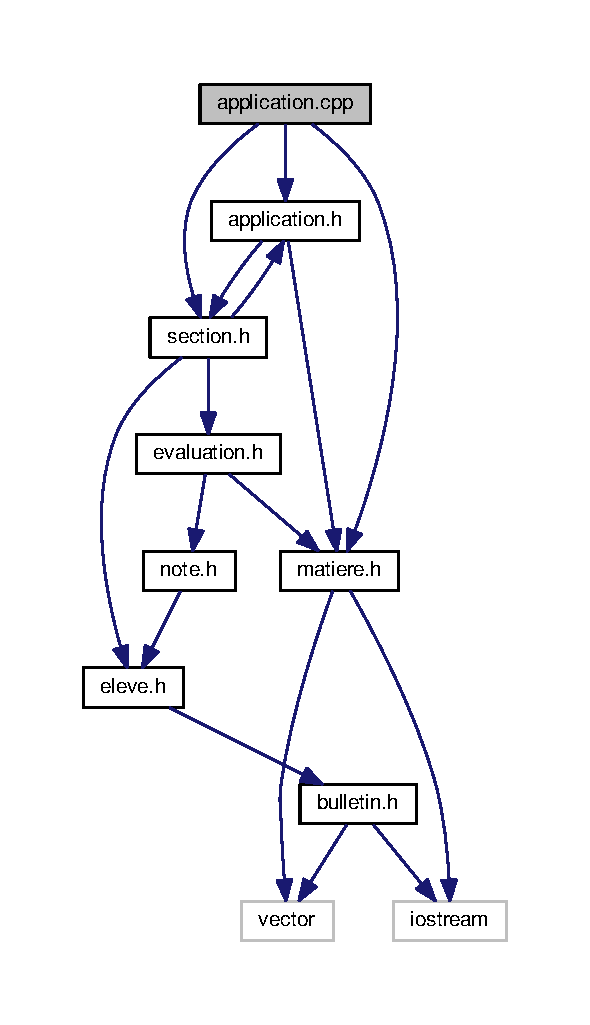
\includegraphics[width=283pt]{application_8cpp__incl}
\end{center}
\end{figure}

\hypertarget{application_8h}{\section{application.\+h File Reference}
\label{application_8h}\index{application.\+h@{application.\+h}}
}
{\ttfamily \#include \char`\"{}section.\+h\char`\"{}}\\*
{\ttfamily \#include \char`\"{}matiere.\+h\char`\"{}}\\*
Include dependency graph for application.\+h\+:\nopagebreak
\begin{figure}[H]
\begin{center}
\leavevmode
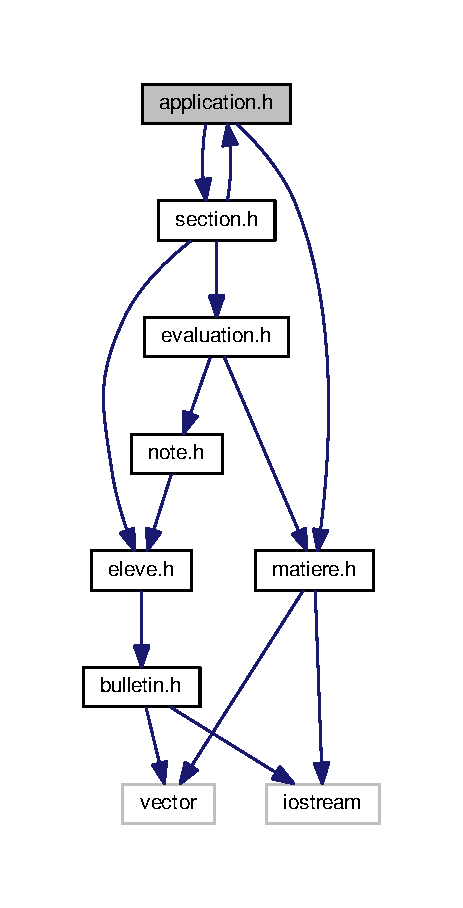
\includegraphics[width=222pt]{application_8h__incl}
\end{center}
\end{figure}
This graph shows which files directly or indirectly include this file\+:\nopagebreak
\begin{figure}[H]
\begin{center}
\leavevmode
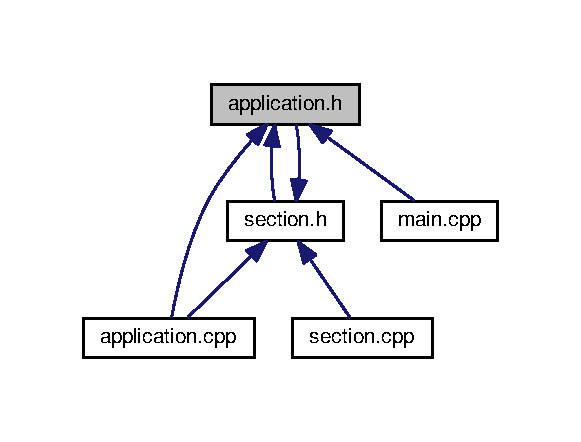
\includegraphics[width=279pt]{application_8h__dep__incl}
\end{center}
\end{figure}
\subsection*{Classes}
\begin{DoxyCompactItemize}
\item 
class \hyperlink{class_application}{Application}
\end{DoxyCompactItemize}


\subsection{Detailed Description}
\begin{DoxyAuthor}{Author}
Courtial Kevin 
\end{DoxyAuthor}
\begin{DoxyVersion}{Version}
0.\+1 
\end{DoxyVersion}

\hypertarget{apreciation_8h}{\section{apreciation.\+h File Reference}
\label{apreciation_8h}\index{apreciation.\+h@{apreciation.\+h}}
}

\hypertarget{bulletin_8h}{\section{bulletin.\+h File Reference}
\label{bulletin_8h}\index{bulletin.\+h@{bulletin.\+h}}
}
{\ttfamily \#include $<$iostream$>$}\\*
{\ttfamily \#include $<$vector$>$}\\*
Include dependency graph for bulletin.\+h\+:\nopagebreak
\begin{figure}[H]
\begin{center}
\leavevmode
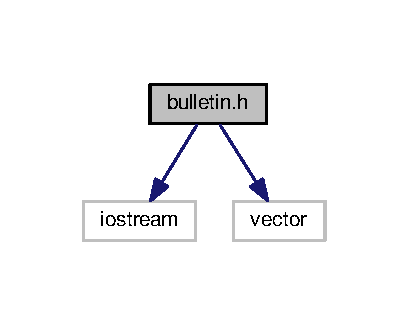
\includegraphics[width=196pt]{bulletin_8h__incl}
\end{center}
\end{figure}
This graph shows which files directly or indirectly include this file\+:\nopagebreak
\begin{figure}[H]
\begin{center}
\leavevmode
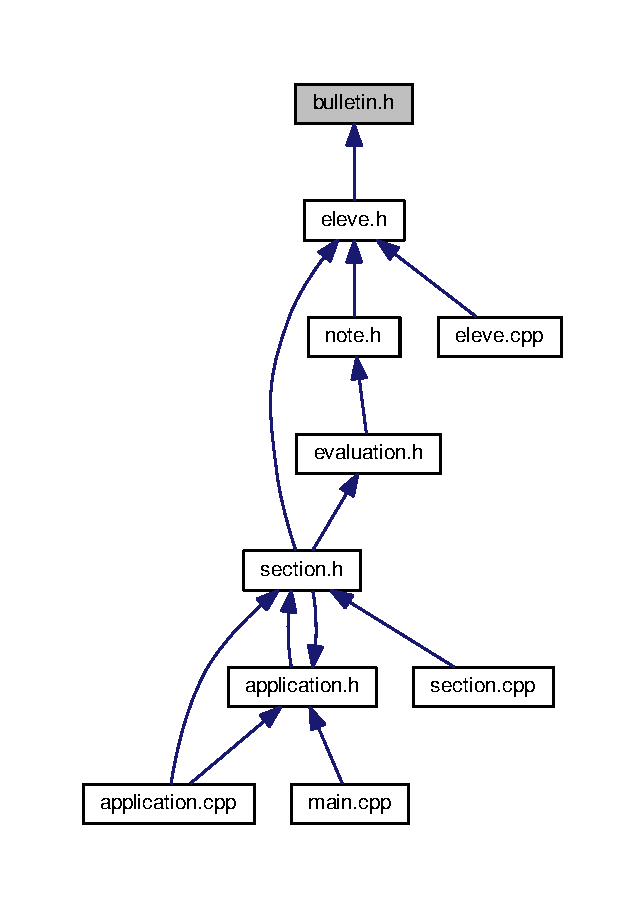
\includegraphics[width=309pt]{bulletin_8h__dep__incl}
\end{center}
\end{figure}
\subsection*{Classes}
\begin{DoxyCompactItemize}
\item 
class \hyperlink{class_bulletin}{Bulletin}
\end{DoxyCompactItemize}

\hypertarget{eleve_8cpp}{\section{eleve.\+cpp File Reference}
\label{eleve_8cpp}\index{eleve.\+cpp@{eleve.\+cpp}}
}
{\ttfamily \#include \char`\"{}eleve.\+h\char`\"{}}\\*
Include dependency graph for eleve.\+cpp\+:\nopagebreak
\begin{figure}[H]
\begin{center}
\leavevmode
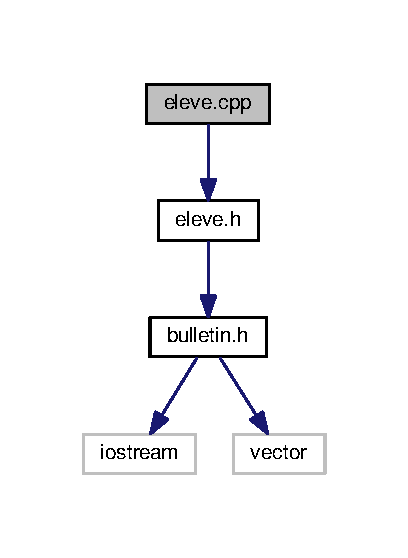
\includegraphics[width=196pt]{eleve_8cpp__incl}
\end{center}
\end{figure}

\hypertarget{eleve_8h}{\section{eleve.\+h File Reference}
\label{eleve_8h}\index{eleve.\+h@{eleve.\+h}}
}
{\ttfamily \#include \char`\"{}bulletin.\+h\char`\"{}}\\*
Include dependency graph for eleve.\+h\+:\nopagebreak
\begin{figure}[H]
\begin{center}
\leavevmode
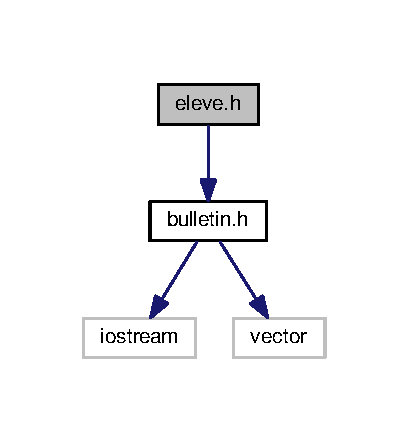
\includegraphics[width=196pt]{eleve_8h__incl}
\end{center}
\end{figure}
This graph shows which files directly or indirectly include this file\+:\nopagebreak
\begin{figure}[H]
\begin{center}
\leavevmode
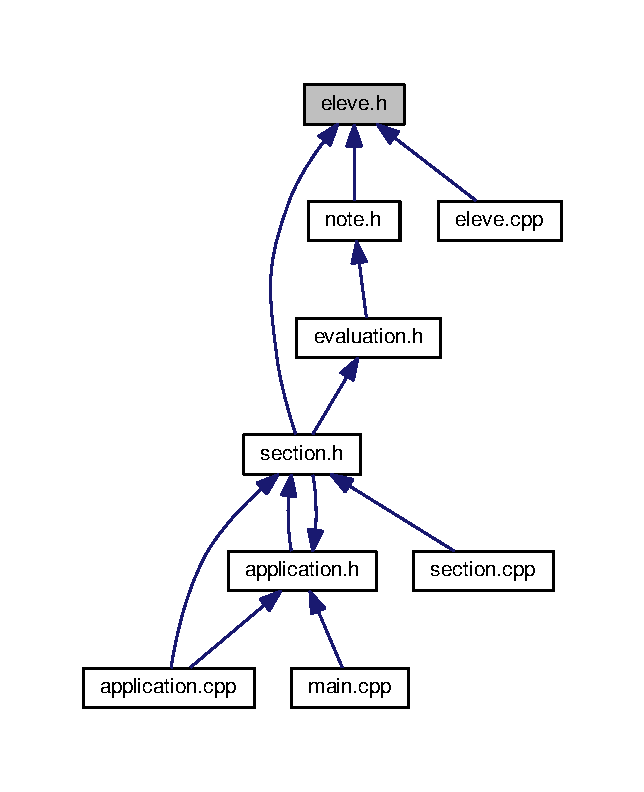
\includegraphics[width=309pt]{eleve_8h__dep__incl}
\end{center}
\end{figure}
\subsection*{Classes}
\begin{DoxyCompactItemize}
\item 
class \hyperlink{class_eleve}{Eleve}
\end{DoxyCompactItemize}

\hypertarget{evaluation_8h}{\section{evaluation.\+h File Reference}
\label{evaluation_8h}\index{evaluation.\+h@{evaluation.\+h}}
}
{\ttfamily \#include \char`\"{}note.\+h\char`\"{}}\\*
{\ttfamily \#include \char`\"{}matiere.\+h\char`\"{}}\\*
Include dependency graph for evaluation.\+h\+:\nopagebreak
\begin{figure}[H]
\begin{center}
\leavevmode
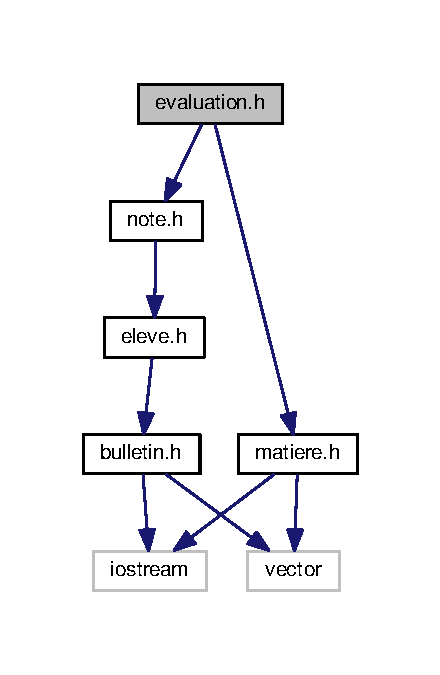
\includegraphics[width=211pt]{evaluation_8h__incl}
\end{center}
\end{figure}
This graph shows which files directly or indirectly include this file\+:\nopagebreak
\begin{figure}[H]
\begin{center}
\leavevmode
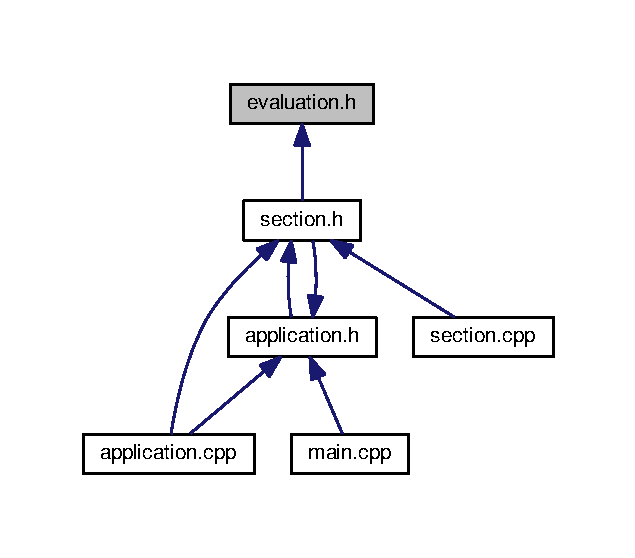
\includegraphics[width=305pt]{evaluation_8h__dep__incl}
\end{center}
\end{figure}
\subsection*{Classes}
\begin{DoxyCompactItemize}
\item 
class \hyperlink{class_evaluation}{Evaluation}
\end{DoxyCompactItemize}

\hypertarget{main_8cpp}{\section{main.\+cpp File Reference}
\label{main_8cpp}\index{main.\+cpp@{main.\+cpp}}
}
{\ttfamily \#include \char`\"{}application.\+h\char`\"{}}\\*
Include dependency graph for main.\+cpp\+:\nopagebreak
\begin{figure}[H]
\begin{center}
\leavevmode
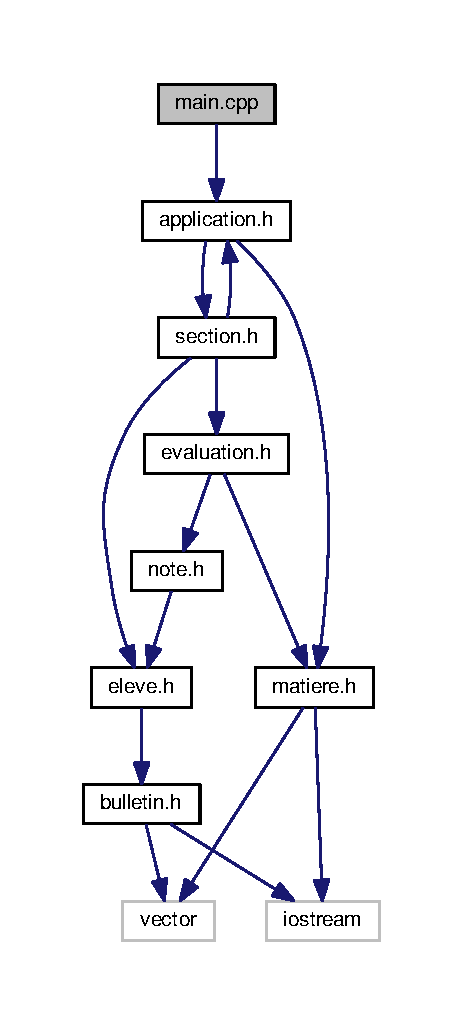
\includegraphics[width=222pt]{main_8cpp__incl}
\end{center}
\end{figure}
\subsection*{Functions}
\begin{DoxyCompactItemize}
\item 
int \hyperlink{main_8cpp_ae66f6b31b5ad750f1fe042a706a4e3d4}{main} ()
\end{DoxyCompactItemize}


\subsection{Function Documentation}
\hypertarget{main_8cpp_ae66f6b31b5ad750f1fe042a706a4e3d4}{\index{main.\+cpp@{main.\+cpp}!main@{main}}
\index{main@{main}!main.\+cpp@{main.\+cpp}}
\subsubsection[{main}]{\setlength{\rightskip}{0pt plus 5cm}int main (
\begin{DoxyParamCaption}
{}
\end{DoxyParamCaption}
)}}\label{main_8cpp_ae66f6b31b5ad750f1fe042a706a4e3d4}

\hypertarget{matiere_8cpp}{\section{matiere.\+cpp File Reference}
\label{matiere_8cpp}\index{matiere.\+cpp@{matiere.\+cpp}}
}
{\ttfamily \#include \char`\"{}matiere.\+h\char`\"{}}\\*
Include dependency graph for matiere.\+cpp\+:\nopagebreak
\begin{figure}[H]
\begin{center}
\leavevmode
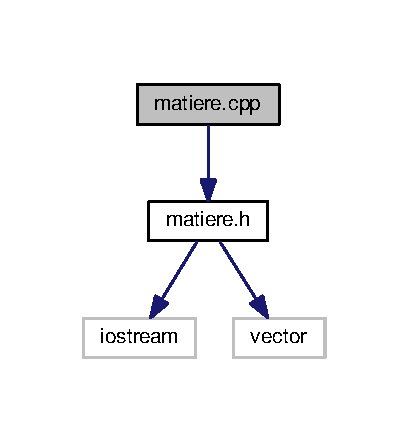
\includegraphics[width=196pt]{matiere_8cpp__incl}
\end{center}
\end{figure}

\hypertarget{matiere_8h}{\section{matiere.\+h File Reference}
\label{matiere_8h}\index{matiere.\+h@{matiere.\+h}}
}
{\ttfamily \#include $<$iostream$>$}\\*
{\ttfamily \#include $<$vector$>$}\\*
Include dependency graph for matiere.\+h\+:\nopagebreak
\begin{figure}[H]
\begin{center}
\leavevmode
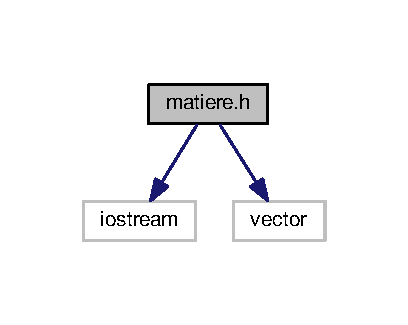
\includegraphics[width=196pt]{matiere_8h__incl}
\end{center}
\end{figure}
This graph shows which files directly or indirectly include this file\+:\nopagebreak
\begin{figure}[H]
\begin{center}
\leavevmode
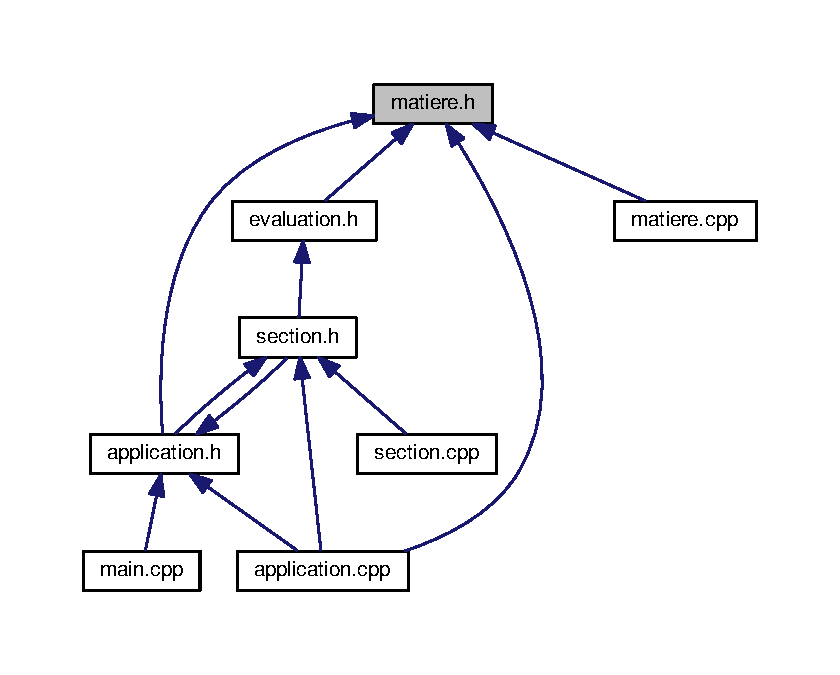
\includegraphics[width=350pt]{matiere_8h__dep__incl}
\end{center}
\end{figure}
\subsection*{Classes}
\begin{DoxyCompactItemize}
\item 
class \hyperlink{class_matiere}{Matiere}
\end{DoxyCompactItemize}

\hypertarget{note_8h}{\section{note.\+h File Reference}
\label{note_8h}\index{note.\+h@{note.\+h}}
}
{\ttfamily \#include \char`\"{}eleve.\+h\char`\"{}}\\*
Include dependency graph for note.\+h\+:\nopagebreak
\begin{figure}[H]
\begin{center}
\leavevmode
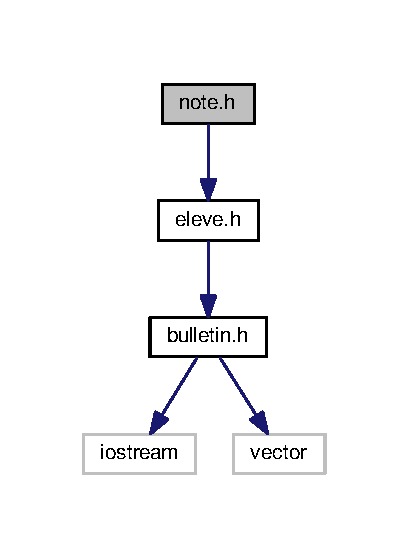
\includegraphics[width=196pt]{note_8h__incl}
\end{center}
\end{figure}
This graph shows which files directly or indirectly include this file\+:\nopagebreak
\begin{figure}[H]
\begin{center}
\leavevmode
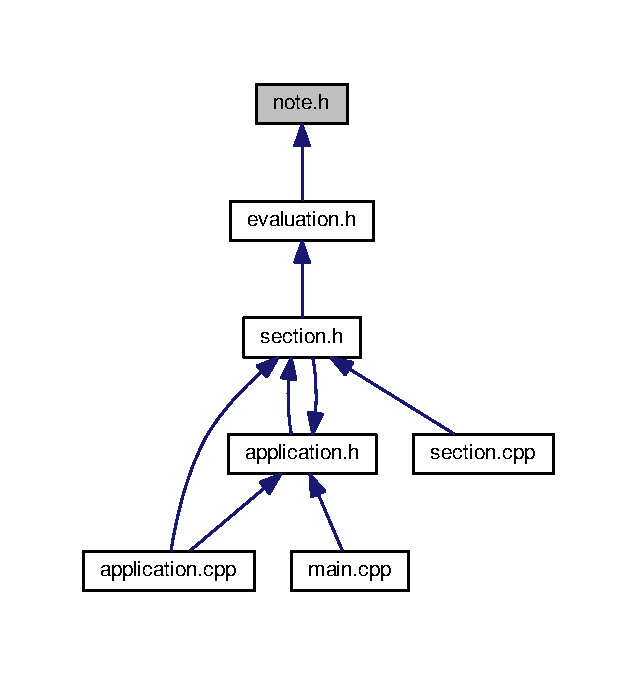
\includegraphics[width=305pt]{note_8h__dep__incl}
\end{center}
\end{figure}
\subsection*{Classes}
\begin{DoxyCompactItemize}
\item 
class \hyperlink{class_note}{Note}
\end{DoxyCompactItemize}

\hypertarget{section_8cpp}{\section{section.\+cpp File Reference}
\label{section_8cpp}\index{section.\+cpp@{section.\+cpp}}
}
{\ttfamily \#include \char`\"{}section.\+h\char`\"{}}\\*
Include dependency graph for section.\+cpp\+:\nopagebreak
\begin{figure}[H]
\begin{center}
\leavevmode
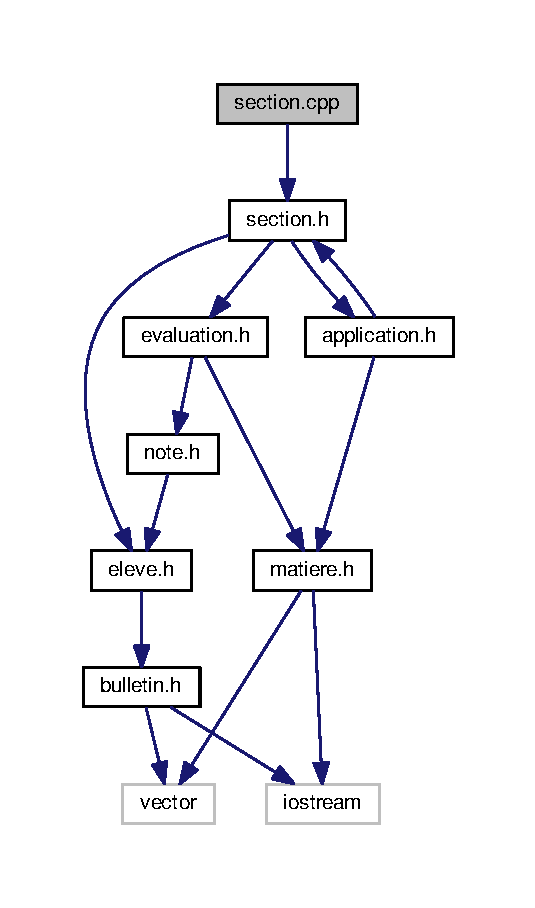
\includegraphics[width=257pt]{section_8cpp__incl}
\end{center}
\end{figure}

\hypertarget{section_8h}{\section{section.\+h File Reference}
\label{section_8h}\index{section.\+h@{section.\+h}}
}
{\ttfamily \#include \char`\"{}eleve.\+h\char`\"{}}\\*
{\ttfamily \#include \char`\"{}evaluation.\+h\char`\"{}}\\*
{\ttfamily \#include \char`\"{}application.\+h\char`\"{}}\\*
Include dependency graph for section.\+h\+:\nopagebreak
\begin{figure}[H]
\begin{center}
\leavevmode
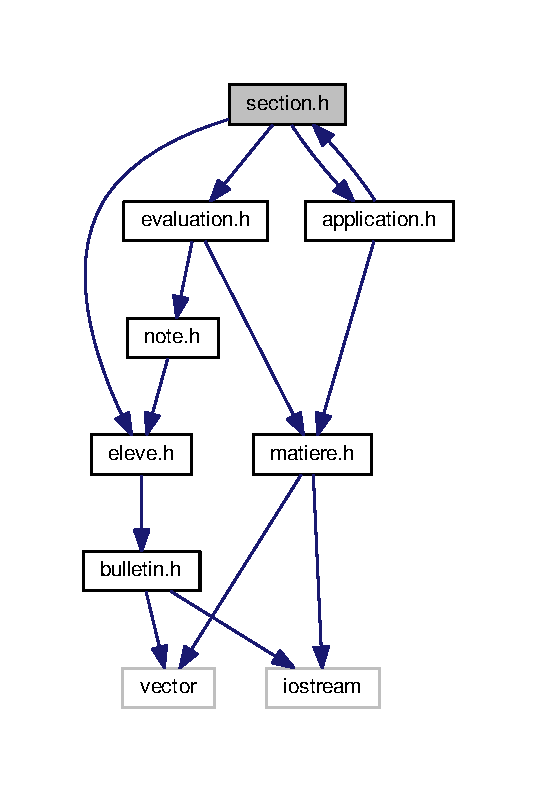
\includegraphics[width=257pt]{section_8h__incl}
\end{center}
\end{figure}
This graph shows which files directly or indirectly include this file\+:\nopagebreak
\begin{figure}[H]
\begin{center}
\leavevmode
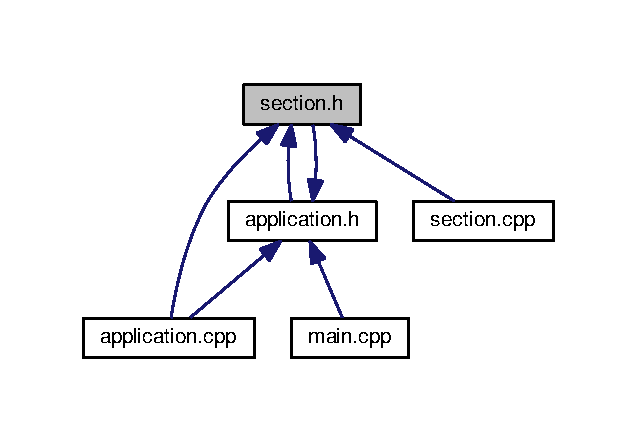
\includegraphics[width=305pt]{section_8h__dep__incl}
\end{center}
\end{figure}
\subsection*{Classes}
\begin{DoxyCompactItemize}
\item 
class \hyperlink{class_section}{Section}
\end{DoxyCompactItemize}

%--- End generated contents ---

% Index
\newpage
\phantomsection
\addcontentsline{toc}{chapter}{Index}
\printindex

\end{document}
